\documentclass[12pt]{article}

\usepackage[utf8]{inputenc}
\usepackage[brazil]{babel}
\usepackage{amsmath, amssymb}
\usepackage{geometry}
\usepackage{graphicx}
\usepackage{enumitem}
\usepackage{tikz}
\usetikzlibrary{tikzmark}
\usepackage{tabularx}
\usepackage{makecell}
\usepackage{array}
\usepackage{pdflscape}
\usepackage{amssymb}
\usepackage{multicol}
\usepackage{pgfplots}
\pgfplotsset{compat=1.18}
\setlength{\columnsep}{0.7cm}
\usetikzlibrary{intersections}
\usetikzlibrary{shapes.geometric, arrows.meta}
\usetikzlibrary{arrows.meta, positioning, shapes.misc, fit, calc}
\usetikzlibrary{positioning, arrows.meta}
\usepackage[most]{tcolorbox}
\usepackage{hyperref}
\usepackage{subcaption} 
\usepackage{caption}
\usepackage{float}

\tcbset{
  mynote/.style={
    colback=gray!10,
    colframe=gray!80,
    fonttitle=\bfseries,
    coltitle=black,
    boxrule=0.5pt,
    arc=4pt,
    left=6pt,
    right=6pt,
    top=4pt,
    bottom=4pt
  }
}
\geometry{a4paper, margin=2.5cm}

\title{Apostila de Circuitos Digitais}
\author{%
    Nathalie Godoi, Julia Acras, Isabella Stuart, Rafaela Leitoles\\
    \vspace{0.2cm}
    \large PET Computação UFPR\\
    \large Tutor: Luiz Carlos Pessoa Albini
}
\date{20/02/2026}

\begin{document}

\maketitle

\tableofcontents
\clearpage

\section{Números binários}

\subsection{Bytes}
\begin{itemize}
    \item Cada dígito de um número armazenado é chamado de \textbf{\textit{bit}} (\textit{binary digit}).
    \item Um conjunto de 4 \textit{bits} é chamado de \textbf{\textit{nibble}}.
    \begin{itemize}
        \item [""] Ele é útil quando manipulamos valores em hexadecimal.
    \end{itemize}
    \item Um conjunto de 8 \textit{bits} é chamado de \textbf{\textit{byte}}.
    \begin{itemize}
        \item [""] Na maioria das CPUs, é a menor unidade utilizada para operações.
    \end{itemize}
\end{itemize}

\subsection{Bases numéricas}
No cotidiano, utilizamos números compostos por algarismos de 0 a 9. Como isso equivale a um total de 10 algarismos, chamamos de \textbf{base decimal} (ou base 10).
\begin{itemize}
    \item Você também conhece a base 2, também chamada de base binária, porque possui 2 algarismos válidos: 0 e 1.
\end{itemize}
Vale ressaltar que isso se aplica a \textbf{qualquer valor}. Logo, é possível utilizar um sistema numérico de base 7, por exemplo. Para isso, basta serem utilizados somente 7 algarismos.

\begin{tcolorbox}[mynote, title= Observação]
Devido ao sistema numérico que utilizamos no dia a dia, a escolha mais intuitiva seria usar algarismos de 0 a 6 para representar essa base. Mas, é importante destacar que \textbf{quaisquer símbolos} poderiam ser utilizados para representar esses valores.
\end{tcolorbox}
\vspace{0.2cm}
\textbf{Bases numéricas mais utilizadas: }
\begin{multicols}{2}
\begin{itemize}
    \item $b_{2} =$ \textbf{binária} (de 0 a 1)
    \item $b_{4} =$ \textbf{\textit{nimble}} (de 0 a 3)
    \columnbreak
    \item $b_{8} =$ \textbf{octal } (de 0 a 7)
    \item $b_{16} =$ \textbf{hexadecimal} (de 0 a 15)
\end{itemize}
\end{multicols}
\noindent Para a representação dos valores de 10 a 15 na base hexadecimal, utilizamos letras de $A$ a $F$. Dessa forma,
\begin{itemize}
    \item $b_{16} \in \{0, 1, 2, 3, 4, 5, 6, 7, 8, 9, A, B, C, D, E, F\}$
\end{itemize}

\subsection{Sistema posicional}
Considerando um número qualquer na base decimal, como 1325. Note que ele é composto da seguinte maneira:
\begin{itemize}
    \item [""] $1325 = 1000 + 300 + 20 + 5 = 1 \times 10^{3} + 3 \times 10^{2} + 2 \times 10^{1} + 5 \times 10^{0}$
    \item Conclusão: a cada casa avançada para a esquerda, é \textbf{multiplicado por 10} o peso do algarismo na soma total.
\end{itemize}
Isso é o que chamamos de \textbf{sistema posicional}: cada algarismo está numa posição, que vai de 0 até n, da direita para a esquerda. Quanto mais à esquerda, \textbf{mais significativo} ele é, isto é, maior a sua influência sobre a soma total.
\vspace{0.2cm} \\
No caso do 1325: as posições vão de 0 a 3, da seguinte maneira: $\underset{3\,2\,1\,0}{1325}$
\begin{itemize}
    \item Algarismo mais significativo = 1
    \item Algarismo menos significativo = 5
\end{itemize}
Note que os valores das posições de cada algarismo coincidem com os expoentes de 10:
\begin{itemize}
    \item $1 \times 10^{3} + 3 \times 10^{2} + 2 \times 10^{1} + 5 \times 10^{0}$
\end{itemize}
Isso também se aplica a números racionais. Considerando o número 124,36:
\begin{itemize}
    \item [""] $124,36 = 100 + 20 + 4 + 0,3 + 0,06$
    \item [""] $124{,}36 = 1 \times 10^{2} + 2 \times 10^{1} + 4 \times 10^{0} + 3 \times 10^{-1} + 6 \times 10^{-2}$
\end{itemize}
De maneira geral, isso se aplica a qualquer base numérica. O que varia entre as bases é o \textbf{valor que multiplica o peso} de cada algarismo, à medida que se avança para a esquerda.
\begin{itemize}
    \item Esse valor sempre será equivalente ao número de algarismos da base numérica utilizada.
    \item [""] Exemplos:
    \begin{itemize}
        \item $362_{7} = 3 \times 7^{2} + 6 \times 7^{1} + 2 \times 7^{0}$
        \item $1010_{2} = 1 \times 2^{3} + 0 \times 2^{2} + 1 \times 2^{1} + 0 \times 2^{0}$
    \end{itemize}
\end{itemize}

\subsection{Conversão de bases}
\vspace{0.2cm}
\subsubsection{Conversão de uma base qualquer para base 10}
Agora que conhecemos o sistema posicional, temos um método direto para converter números de qualquer base para a base decimal ($b_{x} \rightarrow{} b_{10}$). Para isso, basta resolver o polinômio.
\vspace{0.2cm} \\
Exemplos:
\begin{itemize}
\item Convertendo 362 da base 7 para a base decimal ($b_{7} \rightarrow{} b_{10}$):
    \begin{itemize}
        \item [""] $362_{7} = 3 \times 7^{2} + 6 \times 7^{1} + 2 \times 7^{0}$
        \item [""] $362_{7} = 147 + 42 + 2$
        \item [""] $362_{7} = 191_{10}$
    \end{itemize}
\item [""] \textbf{Resposta: 191}.
\item Convertendo 1010 da base binária para a base decimal ($b_{2} \rightarrow{} b_{10}$):
    \begin{itemize}
        \item [""] $1010_{2} = 1 \times 2^{3} + 0 \times 2^{2} + 1 \times 2^{1} + 0 \times 2^{0}$
        \item [""] $1010_{2} = 8 + 0 + 2 + 0$
        \item [""] $1010_{2} = 10_{10}$
    \end{itemize}
\item [""] \textbf{Resposta: 10}.
\end{itemize}
\subsubsection{Conversão da base 10 para uma base qualquer}
Como exemplo, vamos converter $29$ para binário. Temos que:
\begin{itemize}
    \item [""] $29_{10} = 16 + 8 + 4 + 1$
    \item [""] $29_{10} = 1 \times 2^{4} + 1 \times 2^{3} + 1 \times 2^{2} + 1 \times 2^{0}$
    \item [""] $29_{10} = 1 \times 2^{4} + 1 \times 2^{3} + 1 \times 2^{2} + 0 \times 2^{1} + 1 \times 2^{0}$
    \item [""] $29_{10} = 11101_{2}$
\end{itemize}
Ou seja, o raciocínio consiste em descobrir quais potências de 2 somadas resultam no valor desejado.
\begin{multicols}{2}
\raggedcolumns
\vspace*{0.12cm}
Na prática, a maneira mais fácil de descobri-las é dividindo o valor sucessivamente por 2, enquanto for possível, e unindo o quociente aos restos, nessa ordem.
\begin{itemize}
    \item Resposta: $29_{10} = 011101_{2}$ ou $11101_{2}$.
\end{itemize}
\columnbreak
% Aqui terá a imagem da divisão
\centering
\begin{tikzpicture}[yscale=0.8, xscale=1.15, font=\sffamily, thick]
    \node at (0.5,0) {29};
    \node at (1.35,0) {2};
    \node at (1.35,-0.85) {14};
    \node at (2.2,-0.85) {2};
    \node at (2.2,-1.7) {7};
    \node at (3.05,-1.7) {2};
    \node at (3.05,-2.55) {3};
    \node at (3.9,-2.55) {2};
    \node at (3.9,-3.4) {1};
    \node at (4.75,-3.4) {2};
    \node at (0.5,-0.85) {1};
    \node at (1.35,-1.7) {0};
    \node at (2.2,-2.55) {1};
    \node at (3.05,-3.4) {1};
    \node at (3.9,-4.25) {1};
    \node at (4.75,-4.25) {0};
    \draw [line width=1.5pt] (-0.2,-0.85) -- (3.9,-4.9) -- (5.175, -4.9);
    \fill [black] (-0.2, -1.17) -- (0.05,-0.85) -- (-0.2,-0.85) -- (-0.2, -1.17);
    \draw [line width=1.1pt] (0.925,0.25) -- (0.925,-0.3) -- (1.775,-0.3);
    \draw [line width=1.1pt] (1.775,-0.6) -- (1.775,-1.15) -- (2.625,-1.15);
    \draw [line width=1.1pt] (2.625,-1.45) -- (2.625,-2.0) -- (3.475,-2.0);
    \draw [line width=1.1pt] (3.475,-2.3) -- (3.475,-2.85) -- (4.325,-2.85);
    \draw [line width=1.1pt] (4.325,-3.15) -- (4.325,-3.7) -- (5.175,-3.7);
\end{tikzpicture}
\end{multicols}
\noindent De maneira geral, esse método funciona para converter números da \textbf{base decimal para qualquer base}: para uma base x, divida-o por x enquanto for possível, e o resultado será a união do quociente aos restos das divisões.

\begin{multicols}{2}
\raggedcolumns
Vamos converter o número $29$ para a base $7$:
\begin{itemize}
    \item [""] $29_{10} = 28 + 1$
    \item [""] $29_{10} = 4 \times 7^{1} + 1 \times 7^{0}$
    \item [""] $29_{10} = 41_{7}$
\end{itemize}
\columnbreak
\vspace*{0.03cm}
\begin{center}
\begin{tikzpicture}[scale=1.3, yscale=0.8, xscale=1.3, font=\sffamily\Large, thick]
    \node at (0.5,0) {29};
    \node at (1.35,0) {7};
    \node at (1.35,-0.85) {4};
    \node at (2.2,-0.85) {7};
    \node at (2.2,-1.7) {0};
    \node at (0.5,-0.85) {1};
    \node at (1.35,-1.7) {4};
    \draw [line width={1.87 pt}] (0.925,0.25) -- (0.925,-0.3) -- (1.775,-0.3);
    \draw [line width={1.87 pt}] (1.775,-0.6) -- (1.775,-1.15) -- (2.625,-1.15);
\end{tikzpicture}
\end{center}
\end{multicols}
\subsubsection{Conversão da base 10 para base 2, para números racionais}
Voltemos à representação de um número racional, com base no sistema posicional:
\begin{itemize}
    \item [""] $20{,}375_{10} = 2 \times 10^{1} + 0 \times 10^{0} + 3 \times 10^{-1} + 7 \times 10^{-2} + 5 \times 10^{-3}$
\end{itemize}
Convertendo $20,375_{10}$ para binário:
\begin{itemize}
    \item [""] $20,375 = 20 + 0,375$
    \item [""] Como visto anteriormente,
    \begin{itemize}
        \item [""] $20 = 16 + 4 = 1 \times 2^{4} + 1 \times 2^{2}$
        \item [""] $20 = 1 \times 2^{4} + 0 \times 2^{3} + 1 \times 2^{2} + 0 \times 2^{1} + 0 \times 2^{0}$
        \item [""] $20_{10} = 10100_{2}$
    \end{itemize}
\end{itemize}

\newpage
\noindent
Agora, convertendo $0,375$:
\begin{itemize}
    \item Sendo $F$ a parte fracionária de um racional, tal que $0 < F < 1$.
    \begin{itemize}
        \item [""] Nesse caso, teremos $F = 0,375$.
    \end{itemize}
    \item A representação de $F$ na base 2 será:
    \begin{itemize}
        \item [""] $F = b_{1} \times 2^{-1} + b_{2} \times 2^{-2} + \dots + b_{n} \times 2^{-n}$
    \end{itemize}
    \item [""] Onde $b_{1}, b_{2}, ..., b_{n}$ são os dígitos em binário que queremos encontrar.
    \item Se multiplicarmos ambos os lados dessa equação por 2, teremos:
    \begin{itemize}
        \item [""] $2 \times F = 2 \times [b_{1} \times 2^{-1} + b_{2} \times 2^{-2} + b_{3} \times 2^{-3} + \dots + b_{n} \times 2^{-n}]$
        \item [""] $2 \times F = b_{1} \times 2^{0} + b_{2} \times 2^{-1} + b_{3} \times 2^{-2} + \dots + b_{n} \times 2^{-(n-1)}$
        \item [""] $2 \times F = b_{1} + [b_{2} \times 2^{-1} + b_{3} \times 2^{-2} + \dots + b_{n} \times 2^{-(n-1)}]$
        \item [""] $2 \times F = b_{1} + [b_{2} \times \frac{1}{2} + b_{3} \times \frac{1}{4} + \dots + b_{n} \times \frac{1}{2^{n-1}}]$
    \end{itemize}
    \item [""] Assim, como $b_{x} \in \{0, 1\}$, para todo $x$, a expressão $[b_{2} \times \frac{1}{2} + b_{3} \times \frac{1}{4} + \dots + b_{n} \times \frac{1}{2^{n-1}}]$ será estritamente menor que 1.
    \item Por isso, podemos concluir que $2 \times F$ equivale à soma entre uma parte inteira (nesse caso, $b_{1}$) e uma parte fracionária, e a parte inteira de $2 \times F$ será exatamente o dígito em binário que queremos encontrar.
    \item Logo, para converter um valor racional para binário, basta que esse processo seja repetido: multiplicar $F$ por 2 e subtrair sua parte inteira, enquanto $F > 0$.
    \item Dado esse raciocínio, temos o seguinte algoritmo:
    \begin{verbatim}
    k := 1;
    F := r10; (* parte racional em base 10 *)

    do
        F := F * 2;
        dk := parte_inteira(F);
        F := F - dk;
        k := k + 1;
    while (F > 0);
    \end{verbatim}
    \item [""] Exemplo de execução para $F = 0,375$:
    \begin{verbatim}
    F = 0,375
    1ª iteração (k = 1): F * 2 = 0,75 -> d1 = 0, novo F = 0,75
    2ª iteração (k = 2): F * 2 = 1,50 -> d2 = 1, novo F = 0,50
    3ª iteração (k = 3): F * 2 = 1,00 -> d3 = 1, novo F = 0,00
    FIM!
    Resultado: 0,011
    \end{verbatim}
\end{itemize}

\newpage
\noindent
Por fim, temos:
\begin{itemize}
    \item [""] $20,375_{10} = 20 + 0,375$
    \item [""] $20,375_{10} = 10100_{2} + 0,011_{2}$
    \item [""] $20,375_{10} = 10100,011_{2}$
\end{itemize}

\subsubsection{Conversão de base n para base potência de n}
Quando uma base é potência de outra, existe uma relação direta entre grupos de dígitos na base menor e dígitos únicos na base maior. Utilizando $b_{2}$ e $b_{4}$ como exemplo:
\begin{center}
\begin{tabular}{|c|c|}
\hline
\textbf{Binário} & \textbf{Nimble} \\
\hline
$00_{2}$ & $0_{4}$ \\
\hline
$01_{2}$ & $1_{4}$ \\
\hline
$10_{2}$ & $2_{4}$ \\
\hline
$11_{2}$ & $3_{4}$ \\
\hline
\end{tabular}
\end{center}
Ou seja, para converter valores de uma base a outra, basta dividir o número de \textbf{menor} base em grupos e analisar qual é o dígito correspondente na base maior.
\begin{itemize}
    \item Exemplo 1: convertendo $110100111_{2}$ para $b_{4}$
    \item [""] $\overset{1}{\overbrace{01}}\overset{2}{\overbrace{10}}\overset{2}{\overbrace{10}}\overset{1}{\overbrace{01}}\overset{3}{\overbrace{11}}$
    \item [""] Logo, $110100111_{2}$ = $12213_{4}$.
    \item [""] Aqui, como 4 = $2^2$, o expoente é 2 e o número de base menor (nesse caso, $b_{2}$) é dividido em grupos de 2 dígitos.
    \item Exemplo 2: convertendo $110100111_{2}$ para $b_{8}$
    \item [""] $\overset{6}{\overbrace{110}}\overset{4}{\overbrace{100}}\overset{7}{\overbrace{111}}$
    \item [""] Logo, $110100111_{2}$ = $647_{8}$.
    \item [""] Mesmo raciocínio: como $8 = 2^{3}$, o valor de base 2 é dividido em grupos de 3 dígitos.
\end{itemize}
\begin{tcolorbox}[mynote, title= Observação]
Sempre comece o agrupamento da direita para a esquerda. Se faltarem dígitos para completar algum grupo, preencha com zeros à esquerda. Note que isso foi necessário para a resolução do exemplo 1.
\end{tcolorbox}

\subsubsection{Conversão de base potência de n para base n}
Trata-se do processo inverso: basta selecionar cada dígito do número de \textbf{maior} base e substituí-lo pelo valor correspondente na base menor.

\begin{itemize}
    \item Exemplo: convertendo $52543_{8}$ para $b_{2}$
    \item [""] $52543_{8} = \overset{101}{\overbrace{5}}\overset{010}{\overbrace{2}}\overset{101}{\overbrace{5}}\overset{100}{\overbrace{4}}\overset{011}{\overbrace{3}} = 101010101100011_{2}$
\end{itemize}

\subsection{Exercícios}
\begin{enumerate}
\item \textbf{Converta:}
\begin{multicols}{2}
    \begin{enumerate}
        \item $10110_2$ para a base 10.
        \item $213_4$ para a base 10.
        \item $57_8$ para a base 10.
        \item $1F_{16}$ para a base 10.
        \item $402_5$ para a base 10.
        \item $45$ para a base 2.
        \item $89$ para a base 5.
        \item $120$ para a base 8.
        \item $200$ para a base 16.
        \item $33$ para a base 3.
        \item $0,25$ para a base 2.
        \item $0,625$ para a base 2.
        \item $2,5$ para a base 2.
        \columnbreak
        \item $7,75$ para a base 2.
        \item $0,375$ para a base 2.
        \item $101110_2$ para a base 4.
        \item $110101111_2$ para a base 8.
        \item $10110110_2$ para a base 16.
        \item $12201_3$ para a base 9.
        \item $100101_2$ para a base 8.
        \item $32_4$ para a base 2.
        \item $70_8$ para a base 2.
        \item $A5_{16}$ para a base 2.
        \item $47_9$ para a base 3.
        \item $C_{16}$ para a base 2.
    \end{enumerate}
\end{multicols}
\end{enumerate}

\newpage
\subsection{Operações básicas com números binários}
\subsubsection{Adição}
É idêntica à soma na base 10.
\begin{itemize}
    \item Exemplo:
\end{itemize}
\[
\begin{array}{cccccc}
& \text{\textcircled{\scriptsize1}} & \text{\textcircled{\scriptsize1}} & \text{\textcircled{\scriptsize1}} & & \\
& & 1 & 1 & 1 & 0 \\
+ & & 1 & 0 & 1 & 1 \\
\hline
& 1 & 1 & 0 & 0 & 1 \\
\end{array}
\]
\begin{itemize}
    \item [""] Os valores circulados são chamados de \textbf{\textit{bits} de \textit{carry}}.
    \item [""] Na soma $1 + 1 = 10$, por exemplo, é enviado um \textit{bit} de \textit{carry} para a próxima coluna, assim como acontece nas somas na base 10.
\end{itemize}
\begin{tcolorbox}
Nesse exemplo, enquanto os operandos possuem 4 \textit{bits} (dígitos), o resultado possui 5. Em um programa, isso pode ser um problema, se não houver espaço na memória para armazenar esse \textit{bit} extra.
\vspace{0.2cm} \\
Nesse caso, terá ocorrido o que chamamos de \textbf{\textit{overflow}}, e o bit mais significativo será descartado, gerando um resultado incorreto para a operação (que, nesse exemplo, seria $1001$).
\end{tcolorbox}

\subsubsection{Subtração}
É idêntica à subtração na base 10.
\begin{itemize}
    \item Exemplo:
\end{itemize}
\[\begin{array}{cccccc}
\\
& 1 &  \overset{0}{\not{1}} & \overset{10}{\not{1}} & \overset{1}{0} \\ -
&  & 0 & 1 & 1 \\
\hline
& 1 & 0 & 1 & 1 \\
\end{array}
\]
\begin{itemize}
    \item [""] Aqui, quando "emprestamos"\ $1$ ao $0$, ele se torna $10$, que é $2$ em binário, como demonstrado acima.
\end{itemize}

\subsubsection{Multiplicação}
É idêntica à multiplicação na base 10.
\begin{itemize}
    \item Exemplo:
\end{itemize}
\[\begin{array}{cccccccccc}
& & & & 1 & 1 & 1 & 1 & \\
& & & \times & 1 & 1 & 1 & 1 & \\
\hline
& & & & ^{10}1 & ^11 & 1 & 1 & \\
& &   & ^{11}1 & 1 & 1 & 1 & \\
&  ^{10} & ^{11}1 & 1 & 1 & 1 &   & \\
 ^{1} & 1 & 1 & 1 & 1 &   & \\
\hline
 1 & 1 & 1 & 0 & 0 & 0 & 0 & 1 \\
\end{array}
\]
\begin{itemize}
    \item [""] Embora o \textit{carry} possa ter mais de um \textit{bit}, as operações seguem a mesma lógica.
\end{itemize}

\subsubsection{Divisão}
É idêntica à divisão na base 10.
\begin{itemize}
    \item Exemplo:
\end{itemize}

\begin{center}
\begin{tikzpicture}[yscale=0.96, xscale=1.38, font=\sffamily, thin]
    \node at (0.5,0) {1110};
    \node at (1.35,0) {10};
    \node at (1.35,-0.85) {111};
    \node at (0.26,-0.85) {-10};
    \node at (0.43, -1.7) {011};
    \node at (0.44, -2.55) {-10};
    \node at (0.6, -3.4) {010};
    \node at (0.63, -4.25) {-10};
    \node at (0.7, -5.1) {00};
    \draw [line width={0.9 pt}] (1.06,0.25) -- (1.06,-0.3) -- (1.775,-0.3); % chave da div
    \draw [line width={0.9 pt}] (0.0,-1.275) -- (0.5,-1.275); % primeira div
    \draw [line width={0.9 pt}] (0.18,-2.975) -- (0.7,-2.975); % segunda div
    \draw [line width={0.9 pt}] (0.36,-4.675) -- (0.9,-4.675); % terceira div
    \draw [line width={0.7 pt}] (0.6,-0.4) -- (0.6,-1.275); % primeira seta
    \draw [line width={0.7 pt}] (0.78,-0.4) -- (0.78,-2.975); % segunda seta
    % ponta da primeira seta
    \fill [black] (0.55, -1.275) -- (0.65, -1.275) -- (0.6, -1.35) -- (0.55, -1.275);
    % ponta da segunda seta
    \fill [black] (0.73, -2.975) -- (0.83, -2.975) -- (0.78, -3.05) -- (0.73, -2.975);
\end{tikzpicture}
\end{center}

\subsection{Exercícios}
\begin{enumerate}
\item \textbf{Calcule:}
\begin{multicols}{2}
    \begin{enumerate}
        \item $00011 + 00101$
        \item $1110 + 011$
        \item $00101 + 10101$
        \item $111 + 111$
        \item $1001 + 1010$
        \item $10101 + 1010110$
        \item $111 - 101$
        \item $1110 - 011$
        \item $100100 - 10101$
        \item $1011 - 100$
        \item $11001 - 1010$
        \item $110101 - 1010110$
        \columnbreak
        \item $111 \times 101$
        \item $1110 \times 011$
        \item $100100 \times 10101$
        \item $1011 \times 100$
        \item $11001 \times 1010$
        \item $1110101 \times 1010110$
        \item $110 \div 10$
        \item $1111 \div 101$
        \item $1000 \div 10$
        \item $10101 \div 111$
        \item $11001 \div 101$
        \item $10010 \div 11$
    \end{enumerate}
\end{multicols}
\end{enumerate}

\newpage
\subsection{Representação de números negativos em binário}
Considerando somente valores positivos, o maior número armazenável em um computador de $n$ bits é igual a $2^n - 1$.
\begin{itemize}
    \item [""] Mas, aplicações práticas exigiam também a representação de valores negativos. A solução inicial foi reservar o bit mais significativo para indicar o sinal: positivo = $0$ e negativo = $1$. Isso é chamado de \textbf{\textit{bit} de sinal} ou \textbf{sinal magnitude}.
    \item [""] Seguindo esse raciocínio, metade dessa faixa de $2^n$ elementos seria negativa e metade positiva.
\end{itemize}
Portanto, em um computador de 8 bits, considerando somente números positivos, teríamos $x \in [0, 255]$, enquanto, com negativos, teríamos $x \in [-127, +127]$.

\subsubsection{Complemento de 1}
Foi um método criado como uma tentativa de aplicação do \textit{bit} de sinal. Não é utilizado atualmente, por possuir algumas inconsistências.

\vspace{0.2cm}
\noindent
“\textit{Para representar um valor negativo, basta inverter todos os bits da sua representação positiva.}”
\vspace{0.2cm}

\noindent
Exemplo: $8_{10} = 00001000_{2}$ e $-8_{10} = 11110111_{2}$.
O seu maior problema é o fato de que, seguindo essa lógica, existem representações para $+0$ e $-0$ , que correspondem a $00000000$ e $11111111$, respectivamente.

\begin{itemize}
    \item [""] Isso exigiria uma maior complexidade por parte dos processadores e dos sistemas operacionais, para saber como gerenciar esses sinais (por exemplo: a comparação \verb|if (x = 0)| deveria considerar os dois zeros).
\end{itemize}

\noindent
Além disso, em operações aritméticas utilizando o complemento de 1, o \textit{overflow} deve ser considerado, o que também aumentaria a complexidade dos sistemas. \\
Exemplo: $A - B = A + (-B) + overflow$


\subsubsection{Complemento de 2}
Nesse contexto, esse método foi criado com o intuito de resolver as inconsistências e complexidades do complemento de 1.
\vspace{0.2cm} \\
“\textit{Para representar um valor negativo, basta inverter todos os bits da sua representação positiva \textbf{e somar 1}.}”

\vspace{0.2cm}
\noindent
\textbf{Por que isso resolve o problema?} 

\noindent
Estudamos que, em complemento de 1, tínhamos $+0 = 00000000$ e $-0 = 11111111$.
Agora, vamos corrigir a representação calculando $11111111 + 1$.

\begin{itemize}
    \item [""] Tecnicamente, o resultado deveria ser $100000000$, mas, por conta do \textit{overflow}, o bit mais significativo é descartado, o que resulta em $00000000$, equivalente a $+0$.
    \item [""] Assim, foi possível eliminar a representação do $-0$.
\end{itemize}

\newpage
\noindent
Além disso, fazendo os devidos ajustes nos negativos, percebe-se que é possível a representação de um número a mais: $10000000$.

\begin{itemize}
    \item [""] Se estivéssemos trabalhando com 9 bits, $010000000$ seria igual a $+128$. No entanto, como não é o caso, esse valor deve ser negativo, dado seu bit de sinal.
    \item [""] Considerando que $-127$ equivale a $10000001$, temos:

    \begin{enumerate}
        \item [""] $-127 - 1 = -128$
        \item [""] $-127 + (-1) = -128$
        \item [""] $10000001 + 11111111 = 110000000$
    \end{enumerate}

    \item [""] Por conta do overflow, obtemos $10000000$ como resultado.
\end{itemize}

\noindent
Sendo assim, em complemento de 2, temos  $x \in [-128, +127]$.
\textbf{Esse é o sistema utilizado por todos os computadores atualmente.}

\begin{tcolorbox}[mynote, title= Observação]
Antes de converter um valor \textbf{negativo} para a base decimal, deve-se subtrair 1, corrigindo a soma que foi feita anteriormente. Depois, basta fazer a conversão normal, resolvendo o polinômio obtido com base no sistema posicional, como visto anteriormente.
\end{tcolorbox}

\noindent
\vspace{0.1cm}
Resumindo:

\begin{itemize}
    \item Convertendo positivo para negativo: inverte os dígitos e soma 1;
    \item Convertendo negativo para positivo: subtrai 1 e inverte.
\end{itemize}

\subsection{Exercícios}
\begin{enumerate}
\item \textbf{Calcule, em binário, considerando valores de 8 bits em complemento de 2:}
\begin{multicols}{2}
    \begin{enumerate}
        \item $9 + (-23)$
        \item $17 + (-46)$
        \item $64 + 72$
        \item $64 + (-72)$
        \item $(-127) + (-1)$
        \columnbreak
        \item $(-32) + (-45)$
        \item $(-32) + 45$
        \item $50 + (-78)$
        \item $50 + 78$
        \item $127 + (-1)$
    \end{enumerate}
\end{multicols}
\end{enumerate}

\newpage
\subsection{Representação de números reais}
Os sistemas de representação vistos até agora (inteiros com sinal, complemento de 2) são suficientes para números inteiros, mas e quando precisamos armazenar números muito grandes, muito pequenos ou com casas decimais?

\vspace{0.2cm} 
\noindent
Para isso, na base 10, usamos o que chamamos de \textbf{notação científica}.

\vspace{0.2cm}
\noindent
Exemplos:

\begin{itemize}
    \item $9.461.000.000.000.000 = 9,461 \times 10^{15}$
    \item $0,000000000053 = 5,3 \times 10^{-11}$
\end{itemize}

\subsubsection{Notação científica × Ponto flutuante}
Na base decimal, um número em notação científica é representado como $\pm M \times 10^{\pm E}$, onde:

\begin{itemize}
    \item $M =$ \textbf{mantissa} (ou significando), um valor entre 1 e 9;
    \item $E =$ \textbf{expoente}, indica quantas casas a vírgula deve deslocar.
\end{itemize}

\noindent
Na base binária, a representação funciona da mesma forma. A única diferença está na base do expoente, que é 2, em vez de 10: $\pm M \times 2^{\pm E}$. 
\vspace{0.2cm} \\
Operações para as bases decimal e binária são feitas exatamente da mesma forma. \\ Exemplos:

\begin{itemize}
    \item $2 \times 10^{2} + 7 \times 10^{1} = 2 \times 10^{2} + 0,7 \times 10^{2} = 2,7 \times 10^{2}$
    \item $1,101 \times 2^{3} - 1,1 \times 2^{2} = 1,101 \times 2^{3} - 0,11 \times 2^{3} = 0,111 \times 2^{3} = 1,11 \times 2^{2}$
    \item $(2 \times 10^{2}) \times (3 \times 10^{1}) = (2 \times 3) \times 10^{2+1} = 6 \times 10^{3}$
    \item $(1,11 \times 2^{3}) \div (1,0 \times 2^{1}) = (1,11 \div 1,0) \times 2^{3-1} = 1,11 \times 2^{2}$
\end{itemize}

\vspace{0.2cm} 
\noindent
Mas, era necessária uma forma de representar a notação científica na memória de um computador. Diante disso, foi criada a representação que chamamos de \textbf{ponto flutuante}. Aqui, vamos estudar um dos vários sistemas de ponto flutuante que existem: \textbf{IEEE 754}, utilizado em grande parte dos processadores comerciais atualmente.

\subsubsection{IEEE 754}
Um número em ponto flutuante no padrão IEEE 754 é composto por três campos: sinal, expoente e mantissa. 
\vspace{0.2cm} \\
Assim, temos: 

\begin{itemize}
    \item Sinal: $0 =$ positivo e $1 =$ negativo;
    \item Expoente: armazenado com viés (ou \textit{bias}) para permitir expoentes negativos sem usar complemento de 2 (veremos sobre isso mais adiante).
    \item Mantissa: armazena apenas a parte fracionária, pois o bit inteiro é implícito (1,xxxx...).
\end{itemize}

\begin{tcolorbox}[mynote]
Assim como temos a convenção de manter a parte inteira entre 1 e 9 no sistema de notação científica, em ponto flutuante, definimos a parte inteira como sendo sempre igual a 1. Dizemos que um número está \textbf{normalizado} quando segue essas convenções. \\
Dessa forma, é possível simplificar o sistema, armazenando na mantissa somente a parte fracionária do valor. Chamamos a parte inteira de \textbf{\textit{bit} implícito}.
\end{tcolorbox}

\subsubsection{Expoente com viés (\textit{bias})}
O viés é o número que se localiza no meio da faixa de valores que podem ser representados no expoente (de 0 a $2^{n}-1$, sendo $n$ o número de \textit{bits}). 
\vspace{0.2cm} \\
Assim, o valor do expoente armazenado equivale ao resultado de \textbf{expoente + viés}.
\vspace{0.2cm} \\
Exemplo, considerando viés = 127:

\begin{itemize}
    \item Expoente real = 7 $\rightarrow{}$ expoente armazenado = 7 + 127 = \textbf{134}.
    \item Expoente real = -3 $\rightarrow{}$ expoente armazenado = -3 + 127 = \textbf{124}.
\end{itemize}

\noindent
Utilizamos esse sistema porque ele permite a representação de valores negativos no expoente, sem utilizar complemento de 2, que aqui seria desvantajoso, uma vez que o processador precisaria de lógica extra para interpretar o sinal do expoente.

\subsubsection{Precisão simples e dupla}
Existem dois formatos de representação de flutuantes: precisão simples e precisão dupla. A seguir, observe essa tabela com o número de \textit{bits} destinado a cada campo:

\begin{center}
\begin{tabular}{|c|c|c|c|c|c|}
\hline
\textbf{Formato} & \textbf{Sinal} & \textbf{Expoente} & \textbf{Mantissa} & \textbf{Total} & \textbf{Viés} \\
\hline
Precisão simples (float) & 1 & 8 & 23 & 32 & 127 \\
\hline
Precisão dupla (double) & 1 & 11 & 52 & 64 & 1023 \\
\hline
\end{tabular}
\end{center}

\noindent
Exemplo, em precisão simples: 

\begin{center}
\vspace{0.2cm} 
$\overset{sinal}{\overbrace{1}}\overset{expoente}{\overbrace{10000010}}\overset{mantissa}{\overbrace{10100000000000000000000}}$  
\end{center}

\subsubsection{Casos especiais}
Nem todo número binário no sistema IEE 754 representa um número real comum. Isso acontece em alguns casos específicos:

\begin{itemize}
    \item Underflow ou overflow: quando o valor é pequeno demais ou grande demais para ser armazenado de forma convencional;
    \item Quando a operação matemática é inválida.
\end{itemize}

\noindent
Nesses casos, temos, em precisão simples:

\begin{center}
\begin{tabular}{|c|c|c|c|c|}
\hline
\textbf{Contexto} & \textbf{Valor representado} & \textbf{Expoente} & \textbf{Bit implícito} & \textbf{Mantissa} \\
\hline
\textbf{Normalizado} & $1,... \times 2^{(E-127)}$ & 1 a 254 & 1 & qualquer valor \\
\hline
\textbf{Zero} & 0 & 0 & 0 & 0 \\
\hline
\textbf{Denormalizado} & $0,... \times 2^{(-126)}$ & 0 & 0 & $\neq 0$ \\
\hline
\textbf{Infinito} & Infinito & 255 & - & 0 \\
\hline
\textbf{NaN} & Inválido & 255 & - & $\neq 0$ \\
\hline
\end{tabular}
\end{center}

\subsubsection{Exemplo de conversão para IEEE 754}
Vamos converter $20,375_{10}$ para IEEE 754, com precisão simples.

\begin{enumerate}
    \item Conversão para binário: como visto anteriormente, $20,375_{10} \rightarrow{} 10100,011_{2}$ 
    \item Normalização: $10100,011_{2} \rightarrow{} 1,0100011_{2} \times 2^{4}$ 
    \item Expoente: expoente real = 4 $\rightarrow{}$ expoente armazenado = $4 + 127 = 131_{10} = 10000011_{2}$ 
    \item Mantissa: \textit{bits} após a vírgula = 0100011. Completando com zeros à direita, até 23 bits, temos: 01000110000000000000000
    \item Sinal: positivo = 0
\end{enumerate}

\vspace{0.2cm}
\noindent
Resultado: 

\begin{center}
$\overset{sinal}{\overbrace{0}}\overset{expoente}{\overbrace{10000011}}\overset{mantissa}{\overbrace{01000110000000000000000}}$ 
\end{center}

\begin{tcolorbox}[mynote, title= Observação]
Na mantissa, quando necessário, completamos o valor armazenado com zeros à direita, porque eles não influenciam no resultado. Pense na base decimal: $0,5_{10} = 0,500_{10}$, por exemplo. Lembre-se de que estamos tratando da representação da \textbf{parte fracionária} do valor.
\end{tcolorbox}

\subsection{Exercícios}
\begin{enumerate}
    \item Converta para o formato IEEE 754 (em precisão simples):
        \begin{enumerate}
            \item $18,75_{10}$
            \item $-5,25_{10}$
            \item $0,1_{10}$
            \item $-0,375_{10}$
            \item $42,25_{10}$
            \item $-0,1_{10}$
        \end{enumerate}
    \item Converta os seguintes valores IEEE 754 (32 bits) para a base decimal:
        \begin{enumerate}
            \item $0 \; 10000011 \; 10110000000000000000000$
            \item $1 \; 10000000 \; 01000000000000000000000$
            \item $0 \; 01111111 \; 00000000000000000000000$
            \item $1 \; 01111100 \; 11000000000000000000000$
            \item $0 \; 10000010 \; 11010000000000000000000$
            \item $1 \; 01111101 \;  10100000000000000000000$
        \end{enumerate}
\end{enumerate}

\section{Terminologia e Símbolos}
Nesta seção, apresentamos os principais símbolo usados nas operações booleanas para garantir o entedimento dos conceitos apresentados no texto. 
\begin{center}
\begin{tabular}{|c|l|}
\hline
\textbf{Símbolo} & \textbf{Operação / Descrição} \\
\hline
$+$ & OR (Disjunção Lógica) \\
$\cdot$ & AND (Conjunção Lógica) \\
$\overline{X}$ & NOT (Negação de $X$) \\
$\sum$ & Soma de mintermos (forma canônica disjuntiva) \\
$\prod$ & Produto de maxtermos (forma canônica conjuntiva) \\
\hline
\end{tabular}
\end{center}


\section{Tabela Verdade}
\subsection{Introdução}
A tabela verdade é um quadro que representa todas as possíveis combinações lógicas entre variáveis booleanas. Ela mostra como os valores de entrada (0 ou 1) influenciam a saída de um circuito.

Para construí-la, divide-se a tabela em duas partes: entradas (ou variáveis) e saídas (ou combinações resultantes). A cada nova variável adicionada, o número de combinações dobra, pois cada variável pode assumir dois valores: \(0\) ou \(1\).

Assim, para \( n \) variáveis, o número total de linhas na tabela será \( 2^n \). Por exemplo, com 7 variáveis, temos \( 2^7 = 128 \) combinações possíveis.

\textbf{Observação:} Neste material, utilizamos \( \overline{A} \) para representar a negação da variável \( A \).

\subsection{Construção da Tabela Verdade}
Na Tabela Verdade, as variáveis de entrada são colocadas do lado esquerdo, enquanto a função resultante que representa o circuito aparece à direita.
Por exemplo, na função $f$ definida a partir da variável $A$, colocamos na coluna da esquerda $A$ e, na direita, o resultado, que depende do valor lógico de $A$. Assim, teremos:

\begin{center}
$ f = \overline{A}$
\vspace{0.5em}
\begin{tikzpicture}
   \node[inner sep=0pt] (tabela) {
      \begin{tabular}{|c|c|}
      \hline
      \textbf{A} & \(\overline{A}\) \\
      \hline
      1 & 0 \\
      0 & 1 \\
      \hline
      \end{tabular}
   };

   \draw[->, thick] (-2.5, 0.25) -- (-1.1, 0.25)
      node[left] at (-2.5, 0.25) {\footnotesize \textbf{Variável de entrada (A)}};
   \draw[->, thick] (2.5, 0.25) -- (1.1, 0.25)
      node[right] at (2.5, 0.25) {\footnotesize \textbf{Saída (\(\overline{A}\))}};
\end{tikzpicture}
\end{center}

\subsection{Operações Lógicas}
\begin{itemize}
   \item \textbf{Conjunção (AND) :} \( A \cdot B \) - verdadeiro somente se \( A \) e \( B \) forem verdadeiros.
   \item \textbf{Disjunção (OR):} \( A + B \) - falso somente se \( A\) e \( B \) forem falsos.
   \item \textbf{Negação (NOT):} \( \overline{A} \) - inverte o valor lógico de \( A \).
   \item \textbf{Implicação:} \( A \rightarrow B \) - falso apenas se \( A \) for verdadeiro e \( B \) falso.
   \item \textbf{Bicondicional:} \( A \leftrightarrow B \) - verdadeiro se \( A \) e \( B \) tiverem o mesmo valor lógico.
\end{itemize}

\subsection*{Exemplo de Negação (\textbf{NOT}): }
$ f = \overline{A}$
\begin{center}
\begin{tabular}{|c|c|}
\hline
A & \( \overline{A} \) \\
\hline
1 & 0 \\
0 & 1 \\
\hline
\end{tabular}

\vspace{0.5em}
\textit{$\overline{A}$ tem sempre o valor lógico oposto de $A$.}
\end{center}

\subsection*{Exemplo de Conjunção (\textbf{AND}): }
$ s = A \cdot B$
\begin{center}
\begin{tabular}{|c|c|c|}
\hline
A & B & \( A \cdot B \) \\
\hline
0 & 0 & 0 \\
0 & 1 & 0 \\
1 & 0 & 0 \\
1 & 1 & 1 \\ 
\hline
\end{tabular}

\vspace{0.5em}
\textit{A função só é verdadeira quando $A$ e $B$ são ambos $1$.}
\end{center}

\subsection*{Exemplo de Disjunção (\textbf{OR}):}
$ g = A + B$
\begin{center}
\begin{tabular}{|c|c|c|}
\hline
A & B & \( A + B \) \\
\hline
0 & 0 & 0 \\
0 & 1 & 1 \\
1 & 0 & 1 \\
1 & 1 & 1 \\ 
\hline
\end{tabular}

\vspace{0.5em}
\textit{A função só é verdadeira quando $A$ ou $B$ são $1$.}
\end{center}

\subsection*{Exemplo Composto: Disjunção, Conjunção e Negação:}
Considere a função:
\begin{center}
$h = \overline{A \cdot B} \cdot C$
\end{center}
Para construir a tabela verdade dessa função, primeiro calculamos\( A \cdot B\), depois aplicamos a negação, e, por fim, combinamos esse resultado com \( C \).

\begin{center}
\begin{minipage}{0.44\textwidth}
\begin{tabular}{|c|c|c|c|c|c|}
\hline
A & B & C & \( A \cdot B \) & \( \overline{A \cdot B} \) & \( \overline{A \cdot B} \cdot C \) \\
\hline
0 & 0 & 0 & 0 & 1 & 0 \\
0 & 0 & 1 & 0 & 1 & 1 \\
0 & 1 & 0 & 0 & 1 & 0 \\
0 & 1 & 1 & 0 & 1 & 1 \\
1 & 0 & 0 & 0 & 1 & 0 \\
1 & 0 & 1 & 0 & 1 & 1 \\
1 & 1 & 0 & 1 & 0 & 0 \\
1 & 1 & 1 & 1 & 0 & 0 \\
\hline
\end{tabular}
\end{minipage}%
\hspace{1em}%
\begin{minipage}{0.2\textwidth}
   \vspace{1em}
   \textit{Note que a função $h$ só é verdadeira quando $C$ e $\overline{A \cdot B}$ são ambos verdadeiras.}
\end{minipage}
\end{center}

Essa tabela permite acompanhar passo a passo o cálculo da função \( h \) para todas as combinações possíveis das variáveis \( A \), \( B \) e \( C \).

\begin{tcolorbox}[mynote, title= Observação: números de linhas da Tabela Verdade]
A cada nova variável adicionada à tabela, o número de linhas dessa tabela verdade dobra. Dá para perceber isso comparando, por exemplo, os exemplos 1 e 2 - onde foram adicionadas 2 novas possibilidades - ou então do exemplo 3 para o 4, que aumentaram 4 possibilidade.  
\end{tcolorbox}

\subsection{Exercícios}
1. Construa a Tabela Verdade das funções abaixo e avalie o seu valor lógico:
\begin{enumerate}
    \item $(A \cdot B) + (B \cdot A)$
    \item $(\overline{A} + B) + (\overline{B} \cdot A)$
    \item $(\overline{A + B}) \cdot  (A + \overline{B})$
    \item $(A \cdot (B \cdot C))$
    \item $(A \cdot B) + (A \cdot C) + (B \cdot C)$
    \item $(A + B) \cdot \overline{C}$
    \item $(A + B) + \overline{A}$
    \item $(A \cdot B) + C$
    \item $(A \cdot B) + (B \cdot C)$
    \item $\overline{(A + B)} \cdot A$
    \item $(A \cdot B) + (A + B)$
    \item $(A \cdot B) + (\overline{A} \cdot C) + (\overline{B} \cdot A)$
\end{enumerate}

2. Mostre se as igualdades abaixo são verdadeiras:
\begin{enumerate}
    \item $(A \cdot B) \cdot C =  A \cdot (B \cdot C)$
    \item $(A \cdot B) + ( A + C) = A \cdot (B + C)$
    \item $(A + B) \cdot (C + \overline{A}) = (B + C)$
\end{enumerate}
\section{Álgebra de Boole}

A Álgebra de Boole utiliza apenas dois valores:
\begin{itemize}
   \item Verdadeiro: $1$
   \item Falso: $0$
\end{itemize}

\subsection{Operações Fundamentais}
As três operações fundamentais são:

\begin{enumerate}
   \item \textbf{AND} (E lógico) \\
   A saída da operação \textbf{AND} é verdadeira somente quando todas as entradas são verdadeiras, ou seja, basta que apenas uma entrada seja falsa (0) para tornar todo o circuito falso. 
   \item \textbf{OR} (OU lógico) \\
   A saída é verdadeira se ao menos uma das entradas é verdadeira. Logo, a única situação em que o circuito tem seu valor lógico falso é quando todas as entradas são 0.
   \item \textbf{NOT} (Negação) \\
   A saída é o inverso da entrada. Se a entrada for verdadeira (1), a saída será falsa (0) e vice-versa.
\end{enumerate} 

\begin{tcolorbox}[mynote, title= Observação: Relação com Diagrama de Venn]
As operações booleanas também podem ser representadas por diagramas de Venn:
\begin{itemize}
   \item \textbf{AND} – Interseção entre os conjuntos $A$ e $B$
   \item \textbf{OR} – União dos conjuntos $A$ e $B$
   \item \textbf{NOT} – Complemento do conjunto $A$
\end{itemize}
\end{tcolorbox}

\vspace{0.2cm}

\subsection{Representação na forma de Diagrama de Venn} 
% A + B + C
\begin{center}
\textbf{Diagrama de Venn da expressão $f = A + B + C$}
\end{center}

\vspace{0.3cm}
\begin{center}
\begin{tikzpicture}
   \begin{scope}
      \fill[blue!20] (-1,0) circle (1.5);
      \fill[blue!20] (1,0) circle (1.5);
      \fill[blue!20] (0,1.8) circle (1.5);
   \end{scope}
   \draw (-1,0) circle (1.5) node[left] {$A$};
   \draw (1,0) circle (1.5) node[right] {$B$};
   \draw (0,1.8) circle (1.5) node[above] {$C$};
   \node at (0,-2.5) {\footnotesize Região destacada: $A \cup B \cup C$};
\end{tikzpicture}
\end{center}
\textbf{Explicação:} Nesse exemplo, para que a função $f$ acima tenha valor lógico 1, é preciso que ao menos \textbf{UMA} das variáveis seja verdadeira.
\vspace{0.2cm}

% A.B.C
\begin{center}
\textbf{Diagrama de Venn da função: $f = A \cdot B \cdot C$}
\end{center}

\vspace{0.3cm}
\begin{center}
\begin{tikzpicture}
   \begin{scope}
   \clip (-1,0) circle (1.5);
   \clip (1,0) circle (1.5);
   \clip (0,1.8) circle (1.5);
   \fill[blue!20] (-1,0) circle (1.5); % Área comum a todos
\end{scope}
   \draw (-1,0) circle (1.5) node[left] {$A$};
   \draw (1,0) circle (1.5) node[right] {$B$};
   \draw (0,1.8) circle (1.5) node[above] {$C$};
   \node at (0,-2.5) {\footnotesize Região destacada: $A \cap B \cap C$};
\end{tikzpicture}
\end{center}
\textbf{Explicação:} Diferente do exemplo anterior, para que essa função $f$ seja verdadeira, é preciso que \textbf{TODAS} as variáveis tenham valor lógico 1.
\vspace{0.2cm}

% A + (B . C)
\begin{center}
\textbf{Diagrama de Venn da expressão: $f = A + (B \cdot C)$}
\end{center}

\vspace{0.3cm}

\begin{center}
\begin{tikzpicture}
   \fill[blue!20] (-1,0) circle (1.5); 

   \begin{scope}
   \clip (1,0) circle (1.5);
   \fill[blue!20] (0,1.8) circle (1.5);
\end{scope}

   \draw (-1,0) circle (1.5) node[left] {$A$};
   \draw (1,0) circle (1.5) node[right] {$B$};
   \draw (0,1.8) circle (1.5) node[above] {$C$};

   \node at (0,-2.5) {\footnotesize Região destacada: $A \cup (B \cap C)$};
\end{tikzpicture}
\end{center}
\textbf{Explicação:}
\vspace{0.2cm}

\begin{center}
\textbf{Diagrama de Venn da expressão: $g = \overline{A \cdot B \cdot C}$}
\end{center}

\vspace{0.3cm}

\begin{center}
\begin{tikzpicture}

\draw[black, thick, fill=blue!20] (-2.8,-1.8) rectangle (2.8,3.5);
   \begin{scope}
      \clip (-1,0) circle (1.5);
      \clip (1,0) circle (1.5);
      \clip (0,1.8) circle (1.5);
      \fill[white] (-2.8,-1.8) rectangle (2.8,3.5);
   \end{scope}

   \draw[black, thick] (-1,0) circle (1.5) node[left] {$A$};
   \draw[black, thick] (1,0) circle (1.5) node[right] {$B$};
   \draw[black, thick] (0,1.8) circle (1.5) node[above] {$C$};
   \node at (-2, 2.8) {$U$};

\end{tikzpicture}
\end{center}
\vspace{0.5cm}

\begin{center}
\footnotesize Região destacada: $\overline{A \cap B \cap C}$
\end{center}

\textbf{Explicação:} Esse exemplo é equivalente ao complemento da interseção de todas as variáveis. Por exemplo, se uma função $f$ é determinada por essa interseção, e como visto anteriormente essa expressão só é verdadeira quando todas as variáveis são simultaneamente 1, temos que nossa função $g$ é verdadeira sempre que $f$ for falsa, ou seja, quando ao menos uma das variáveis não for 1.
\vspace{0.5cm}

\section{Expressões, Axiomas e Simplificação}

Sendo \( X, Y\) e \( Z\) variáveis que assumem os valores lógicos 0 e 1, e utilizando os símbolos:
\begin{itemize}
   \item \( + \) para disjunção (OU lógico)
   \item \( \cdot \) para conjunção (E lógico)
   \item \( \overline{X} \) para negação de X
\end{itemize}

As propriedades fundamentais da Álgebra de Boole serão representadas a seguir, separadas pelas operações OR e AND, para facilitar a compreensão.
\subsection{Versão OR (Soma lógica)}

\begin{center}
\begin{tabular}{|l|l|}
\hline
\textbf{Propriedade (OR)} & \textbf{Expressão} \\
\hline
1 - Identidade       & \( X + 0 = X \) \\
2 - Elemento Nulo    & \( X + 1 = 1 \) \\
3 - Idempotência     & \( X + X = X \) \\
4 - Complemento      & \( X + \overline{X} = 1 \) \\
5 - Involução        & \( \overline{\overline{X}} = X \) \\
6 - Comutativa       & \( X + Y = Y + X \) \\
7 - Associativa      & \( (X + Y) + Z = X + (Y + Z) \) \\
8 - Distributiva     & \( X + (Y \cdot Z) = (X + Y)(X + Z) \) \\
9 - Absorção 1       & \( X + X \cdot Y = X \) \\
10 - Absorção 2      & \( X + \overline{X} \cdot Y = X + Y \) \\
11 - Consenso        & \( X \cdot Y + \overline{X} \cdot Z + Y \cdot Z = X \cdot Y + \overline{X} \cdot Z \) \\
12 - De Morgan       & \( \overline{X + Y} = \overline{X} \cdot \overline{Y} \) \\
\hline
\end{tabular}
\end{center}

\vspace{0.5cm}

\subsection{Versão AND (Produto Lógico)}

\begin{center}
\begin{tabular}{|l|l|}
\hline
\textbf{Propriedade (AND)} & \textbf{Expressão} \\
\hline
1 - Identidade       & \( X \cdot 1 = X \) \\
2 - Elemento Nulo    & \( X \cdot 0 = 0 \) \\
3 - Idempotência     & \( X \cdot X = X \) \\
4 - Complemento      & \( X \cdot \overline{X} = 0 \) \\
5 - Involução        & \( \overline{\overline{X}} = X \) \\
6 - Comutativa       & \( X \cdot Y = Y \cdot X \) \\
7 - Associativa      & \( (X \cdot Y) \cdot Z = X \cdot (Y \cdot Z) \) \\
8 - Distributiva     & \( X \cdot (Y + Z) = X \cdot Y + X \cdot Z \) \\
9 - Absorção 1       & \( X \cdot (X + Y) = X \) \\
10 - Absorção 2      & \( X \cdot (\overline{X} + Y) = X \cdot Y \) \\
11 - Consenso        & \( (X + Y)(\overline{X} + Z)(Y + Z) = (X + Y)(\overline{X} + Z) \) \\
12 - De Morgan       & \( \overline{X \cdot Y} = \overline{X} + \overline{Y} \) \\
\hline
\end{tabular}
\end{center}

As propriedades 2, 8, 9 e 11 serão demonstradas com tabelas verdades. As outras ficam a cargo do leitor demonstar.

\section{Demonstração das Propriedades}

\subsection{Propriedade 2: Elemento Nulo}

Versão OR:
Essa propriedade diz que: 
\[
X + 1 = 1
\]
Veja a tabela verdade a seguir que comprova a igualdade
\begin{center}
\begin{tabular}{|c|c|}
\hline
$X$  & $X + 1$ \\
\hline
0 & 1 \\
1 & 1 \\
\hline
\end{tabular}
\end{center}

Assim, independente do valor lógico de $X$ a função sempre 1.

Versão AND: 
\begin{center}
\begin{tabular}{|c|c|}
\hline
$X$  & $X \cdot 0$ \\
\hline
0 & 0 \\
1 & 0 \\
\hline
\end{tabular}
\end{center}

Dessa forma, fica perceptível que o valor lógico de $X$ na função não altera o valor da função, que será sempre 0.

\subsection{Propriedade 8: Distributiva}

Versão OR:
\begin{center}
\begin{tabular}{|c|c|c|c|c|}
\hline
$X$  & $Y$ & $Z$ & $X + (Y \cdot Z)$ & $(X + Y) \cdot (X + Z)$ \\
\hline
0 & 0 & 0 & 0 & 0 \\
0 & 0 & 1 & 0 & 0 \\
0 & 1 & 0 & 0 & 0 \\
0 & 1 & 1 & 1 & 1 \\
1 & 0 & 0 & 1 & 1 \\
1 & 0 & 1 & 1 & 1 \\
1 & 1 & 0 & 1 & 1 \\
1 & 1 & 1 & 1 & 1 \\
\hline 
\end{tabular}
\end{center}


Versão AND:
\begin{center}
\begin{tabular}{|c|c|c|c|c|}
\hline
$X$  & $Y$ & $Z$ & $X \cdot (Y + Z)$ & $(X \cdot Y) + (X \cdot Z)$ \\
\hline
0 & 0 & 0 & 0 & 0 \\
0 & 0 & 1 & 0 & 0 \\
0 & 1 & 0 & 0 & 0 \\
0 & 1 & 1 & 0 & 0 \\
1 & 0 & 0 & 0 & 0 \\
1 & 0 & 1 & 1 & 1 \\
1 & 1 & 0 & 1 & 1 \\
1 & 1 & 1 & 1 & 1 \\
\hline
\end{tabular}
\end{center}

\subsection{Propriedade 9: Absorção 1}

Versão OR:
\begin{center}
\begin{tabular}{|c|c|c|}
\hline
$X$  & $Y$ & $X + (X \cdot  Y)$ \\
\hline
0 & 0 & 0 \\
0 & 1 & 0 \\
1 & 0 & 1 \\
1 & 1 & 1 \\
\hline
\end{tabular}
\end{center}

Versão AND:
\begin{center}
\begin{tabular}{|c|c|c|}
\hline
$X$  & $Y$ & $X \cdot (X + Y)$ \\
\hline
0 & 0 & 0 \\
0 & 1 & 0 \\
1 & 0 & 1 \\
1 & 1 & 1 \\
\hline
\end{tabular}
\end{center}

\subsection{Propriedade 11: Consensus}

Versão OR:
\begin{center}
\begin{tabular}{|c|c|c|c|c|}
\hline
$X$  & $Y$ & $Z$ & $X \cdot Y + \overline{X} \cdot Z + Y \cdot Z$ & $X \cdot Y + \overline{X} \cdot Z$ \\
\hline
0 & 0 & 0 & 0 & 0 \\
0 & 0 & 1 & 1 & 1 \\
0 & 1 & 0 & 0 & 0 \\
0 & 1 & 1 & 1 & 1 \\
1 & 0 & 0 & 0 & 0 \\
1 & 0 & 1 & 0 & 0 \\
1 & 1 & 0 & 1 & 1 \\
1 & 1 & 1 & 1 & 1 \\
\hline
\end{tabular}
\end{center}

Versão AND:
\begin{center}
\begin{tabular}{|c|c|c|c|c|}
\hline
$X$  & $Y$ & $Z$ &  $(X + Y)(\overline{X} + Z)(Y + Z)$ & $(X + Y)(\overline{X} + Z)$ \\
\hline
0 & 0 & 0 & 0 & 0 \\
0 & 0 & 1 & 0 & 0 \\
0 & 1 & 0 & 1 & 1 \\
0 & 1 & 1 & 1 & 1 \\
1 & 0 & 0 & 0 & 0 \\
1 & 0 & 1 & 1 & 1 \\
1 & 1 & 0 & 1 & 1 \\
1 & 1 & 1 & 1 & 1 \\
\hline
\end{tabular}
\end{center}

\subsection{Exercícios}
Simplifique as expressões abaixo:
\begin{enumerate}
    \item $(A + B) \cdot \overline{A}$
    \item $A + (A \cdot B)$
    \item $(\overline{A} \cdot B) + (X \cdot \overline{D}) + (B \cdot \overline{D}) + (A \cdot \overline{B})$
    \item $(\overline{A} \cdot B \cdot \overline{X}) + (\overline{A} \cdot \overline{B} \cdot \overline{X}) + (A \cdot B \cdot \overline{X}) + (A \cdot \overline{B} \cdot \overline{X})$
    \item $(\overline{A} \cdot B) + (X \cdot \overline{D}) + (B \cdot \overline{D}) + (A \cdot B)$
    \item $(A + \overline{B} + (A \cdot B)) \cdot (A \cdot \overline{B}) \cdot (\overline{A} \cdot B) + D$
    \item $(A + \overline{B} + (A \cdot \overline{B}) + D) \cdot ((A \cdot B) + (\overline{A} \cdot B) + (B \cdot D)) + (\overline{A} + B)$
\end{enumerate}

\section{MINTERMOS E MAXTERMOS}
Mintermos e maxternos são formas canônicas de representar funções booleanas
Toda expressão booleanas pode ser obtida através da sua tabela verdade
\begin{quote}
\textbf{Observação:} Dizemos que uma expressão está na \textit{forma canônica} quando ela é representada por uma \textbf{soma de mintermos} (forma canônica disjuntiva) ou um \textbf{produto de maxtermos} (forma canônica conjuntiva). Em ambas, todas as variáveis da função aparecem em cada termo, direta ou negada.
\end{quote}

\subsection{Mintermos}
Mintermi: é a forma canônica de representar uma linha da tabela verdade utilizando o operador AND (E lógico) entre todas as variáveis da função.
Cada variável pode aparecer de duas formas: direta ou negada, dependendo do valor que ela assume na linha da tabela.

\textit{Notação}: 
\begin{itemize}
   \item Valor 0: a variável aparece \textbf{negada} (exemplo: $A = 0 \Rightarrow \overline{A}$)
   \item Valor 1: a variável aparece \textbf{direta} (exemplo: $A = 1 \Rightarrow A$)
\end{itemize}

O mintermo da primeira linha da tabela verdade é o $m_0$ e o da útima será $m_{2^n - 1}$, sendo $n$ o número de variáveis da função.
Para construir um mintermo, pega-se todas as variáveis da linha e usa-se a operação lógica \textbf{AND} entre elas, respeitando o uso da forma direta ou negada de acordo com os valores. Assim, cada mintermo representa exatamente uma linha onde a saída da função é igual a 1.

\begin{tcolorbox}[mynote, title=Notação – Forma Canônica por Mintermos]
A notação \textit{$f(A, B, C) = \sum m(x, y, z)$} indica que a função $f$ é expressa como uma \textbf{soma de mintermos}, ou seja, uma disjunção (OU) dos termos onde a saída é igual a 1 na tabela verdade. As letras "x", "y" e "z" indicam as \textbf{linhas} que a função é \textbf{1}. 
\end{tcolorbox} 

Construção do Mintermo:
\vspace{0.5cm}
\begin{center}
\begin{tabular}{|c|c|c|c|c|}
\hline
$A$ & $B$ & $C$ & Mintermo &\\
\hline
0 & 0 & 0 & $\overline{A}\cdot\overline{B}\cdot\overline{C}$ & $m_0$ \\
0 & 0 & 1 & $\overline{A}\cdot\overline{B}\cdot C$ & $m_1$ \\
0 & 1 & 0 & $\overline{A}\cdot B\cdot\overline{C}$ & $m_2$ \\
0 & 1 & 1 & $\overline{A}\cdot B\cdot C$ & $m_3$ \\
1 & 0 & 0 & $A\cdot\overline{B}\cdot\overline{C}$ & $m_4$ \\
1 & 0 & 1 & $A\cdot\overline{B}\cdot C$ & $m_5$ \\
1 & 1 & 0 & $A\cdot B\cdot\overline{C}$ & $m_6$ \\
1 & 1 & 1 & $A\cdot B\cdot C$ & $m_7$ \\
\hline
\end{tabular}
\end{center}
\vspace{0.5cm}

\subsection{Maxtermo}
Maxtermo: é a forma canônica de representar uma linha da tabela verdade utilizando o operador OR (OU lógico) entre todas as variáveis da função. 
A contrução dos maxtermos é semlhante à dos mintemos, porém segue a lógica inversa:

\textit{Notação}:
\begin{itemize}
   \item Valor 0: a variável aparece \textbf{direta} (exemplo: $A = 0 \Rightarrow A$)
   \item Valor 1: a variável aparece \textbf{negada} (exemplo: $A = 1 \Rightarrow \overline{A}$)
\end{itemize}

Para cada linha da tabela verdade em que a saída é 0, pode-se formar um maxtermo. O maxtermo da primeira linha da tabela verdade é o $M_0$, e o último será $M_{2^n - 1}$, com $n$ sendo o número de variáveis.

\begin{tcolorbox}[mynote, title=Notação – Forma Canônica por Maxtermos]
A notação \textit{$f(A, B, C) = \prod M(x, y, z)$} indica que a função $f$ é expressa como uma \textbf{produto de maxtermos}, ou seja, uma conjunção (AND) dos termos onde a saída é igual a 0 na tabela verdade. As letras "x", "y" e "z" indicam as \textbf{linhas} que a função é \textbf{zero}.
\end{tcolorbox} 

\vspace{0.5cm}
Construção do Maxtermo:
\begin{center}
\begin{tabular}{|c|c|c|c|c|}
\hline
$A$ & $B$ & $C$ & Mintermo &\\
\hline
0 & 0 & 0 & $A + B + C$ & $M_0$ \\
0 & 0 & 1 & $A + B + \overline{C}$ & $M_1$ \\
0 & 1 & 0 & $A + \overline{B} + C$ & $M_2$ \\
0 & 1 & 1 & $A + \overline{B} + \overline{C}$ & $M_3$ \\
1 & 0 & 0 & $\overline{A} + B + C$ & $M_4$ \\
1 & 0 & 1 & $\overline{A} + B + \overline{C}$ & $M_5$ \\
1 & 1 & 0 & $\overline{A} + \overline{B} + C$ & $M_6$ \\
1 & 1 & 1 & $\overline{A} + \overline{B} + \overline{C}$ & $M_7$ \\
\hline
\end{tabular}
\vspace{0.5cm}
\end{center}

\vspace{0.5cm}

\textbf{Exemplo}:
\[
f = A + B
\]

\begin{center}
\begin{tabular}{|c|c|c|c|c|}
\hline
$A$  & $B$ & $f$ & Mintermo & Maxtermo \\
\hline
0 & 0 & 0 & $m_0 = \overline{A}\overline{B}$ & $M_0 = A + B$ \\
0 & 1 & 1 & $m_1 = \overline{A}B$            & $M_1 = A + \overline{B}$ \\
1 & 0 & 1 & $m_2 = A\overline{B}$            & $M_2 = \overline{A} + B$ \\
1 & 1 & 1 & $m_3 = AB$                       & $M_3 = \overline{A} + \overline{B}$ \\
\hline
\end{tabular}
\end{center}

\begin{itemize}
   \item Os \textbf{mintermos} representam as linhas em que $f = 1$.
   \item Os \textbf{maxtermos} representam as linhas em que $f = 0$.
   \item A função $f = A + B$ tem como forma canônica:
   \begin{itemize}
      \item \textbf{Soma de mintermos:} $f = m_1 + m_2 + m_3 = \overline{A}B + A\overline{B} + AB$
      \item \textbf{Produto de maxtermos:} $f = M_0 = (A + B)$
   \end{itemize}
\end{itemize}

\begin{tcolorbox}[mynote, title={\textbf{Mintermos, Maxtermos e Complemento}}]
Como cada mintermo é o complemento de seu maxtermo correspondente, podemos dizer que o complemento de uma função $f$ é representado pela multiplicação (AND) dos maxtermos associados às linhas onde $f = 0$.

No exemplo acima, como $f = A + B$, temos que $f = 1$ nas linhas 1, 2 e 3, e $f = 0$ apenas na linha 0. Logo, o complemento de $f$ é:

\[
f' = M_0 = A + B
\quad \Rightarrow \quad f = \overline{A + B}
\]

Assim, mostramos que o maxtermo $M_0$ representa exatamente o valor de $f'$ nesta função.
\end{tcolorbox}

\section{Mapa de Karnaugh}
\label{sec:mapaKarnaugh}

O \textbf{Mapa de Karnaugh} (ou \textbf{diagrama de Karnaugh}) é um método gráfico utilizado para simplificar expressões lógicas obtidas a partir de tabelas-verdade. Essa técnica permite realizar a simplificação de forma mais direta e visual, dispensando o uso extensivo das leis algébricas da Álgebra Booleana.

\subsection{Construção do Mapa de Karnaugh}

A forma e o tamanho do Mapa de Karnaugh dependem da quantidade de variáveis envolvidas na expressão lógica, pois o mapa deve representar todas as combinações possíveis entre estas, assim como em uma tabela-verdade.  

O Mapa de Karnaugh pode ser entendido como uma \textit{representação gráfica alternativa} da tabela, organizada para facilitar a identificação de padrões e agrupamentos de termos passíveis de simplificação.

Nesta apostila, abordaremos os mapas de 2, 3 e 4 variáveis, que são os casos mais comuns em aplicações de circuitos digitais.

\subsubsection{Mapa com 2 variáveis}
\label{subsec:2variaveis}

Em um mapa com duas variáveis, a primeira linha e a primeira coluna representam todas as possíveis combinações destas. Assim, o mapa é formado por quatro células, correspondentes aos quatro estados binários possíveis das duas variáveis.  

Cada célula do mapa representa um \textit{mintermo}, conforme explicado anteriormente.

\vspace{0.5cm}

Consideremos uma tabela-verdade com as variáveis \(A\) e \(B\):

\begin{itemize}
    \item Combinações possíveis da variável \(A\): $A$ e $\overline{A}$;
    \item Combinações possíveis da variável \(B\): $B$ e $\overline{B}$.
\end{itemize}

\begin{table}[htb]
\centering
\renewcommand{\arraystretch}{1.3} % espaçamento vertical das células
\begin{tabular}{|c|c|c|}
\hline
 & $\overline{A}$ & $A$ \\
\hline
$\overline{B}$ &  &  \\
\hline
$B$ &  &  \\
\hline
\end{tabular}
\caption{Mapa de Karnaugh para duas variáveis (\(A,B\)).}
\label{tab:karnaugh-2var}
\end{table}

\begin{tcolorbox}[mynote, title=\textbf{Ordem e Disposição das Variáveis}]
A ordem das variáveis no cabeçalho é essencial para a simplificação correta.  
As células são dispostas seguindo o \textbf{código Gray}, isto é, duas células adjacentes diferem em apenas um bit. \\
No mapa de 2 variáveis a sequência na linha/coluna é $\overline{X} \mid X$, sendo \(X\) uma variável arbitrária.  
\end{tcolorbox}

\subsubsection{Mapa com 3 variáveis}
\label{subsec:3variaveis}

Quando temos três variáveis, agrupamos duas delas para compor o eixo horizontal e deixamos a terceira no eixo vertical. Assim, representamos todas as combinações possíveis das três variáveis em um mapa de 8 células — o dobro do mapa de duas variáveis.

\vspace{0.5cm}

Para exemplificar, consideremos as variáveis \(A\), \(B\) e \(C\).  
Aqui agrupamos \(A\) e \(B\) no topo (eixo horizontal) e colocamos \(C\) na lateral esquerda (eixo vertical).

\begin{itemize}
    \item Combinações possíveis de \(A\) e \(B\) (seguindo código Gray): $\overline{A}\overline{B}$, $\overline{A}B$, $AB$, $A\overline{B}$;
    \item Combinações possíveis de \(C\): $\overline{C}$ e $C$.
\end{itemize}

\begin{table}[htb]
\centering
\renewcommand{\arraystretch}{1.3}
\begin{tabular}{|c|c|c|c|c|}
\hline
 & $\overline{A}\overline{B}$ & $\overline{A}B$ & $AB$ & $A\overline{B}$ \\
\hline
$\overline{C}$ &  &  &  &  \\
\hline
$C$ &  &  &  &  \\
\hline
\end{tabular}
\caption{Mapa de Karnaugh para três variáveis (eixo horizontal: \(AB\); eixo vertical: \(C\)).}
\label{tab:karnaugh-3var}
\end{table}

\begin{tcolorbox}[mynote, title=\textbf{Ordem das Variáveis (3 variáveis)}]
A disposição segue a propriedade do código Gray: células adjacentes diferem por apenas um bit.  
Assim, a linha superior tem a ordem $\overline{X}\overline{Y} \mid \overline{X}Y \mid XY \mid X\overline{Y}$, sendo \(X\) e \(Y\) variáveis arbitrárias.  
Para a coluna lateral, aplica-se a mesma sequência de variação de uma única variável apresentada no \hyperref[subsec:2variaveis]{Mapa com 2 variáveis}.
\end{tcolorbox}

\subsubsection{Mapa com 4 variáveis}
\label{subsec:4variaveis}

Quando trabalhamos com quatro variáveis, o mapa é estruturado agrupando duas variáveis no eixo horizontal e as outras duas no eixo vertical.  
A escolha da ordem dos agrupamentos é fundamental para manter a sequência correta do \textbf{código Gray}, o que garante a variação de apenas um bit entre células adjacentes e, consequentemente, facilita o processo de simplificação.

\vspace{0.5cm}

Consideremos as variáveis \(A\), \(B\), \(C\) e \(D\).  
Neste caso, agrupamos \(A\) e \(B\) no eixo horizontal e \(C\) e \(D\) no eixo vertical, conforme mostrado a seguir:

\begin{itemize}
    \item Combinações possíveis de \(A\) e \(B\) (seguindo o código Gray): $\overline{A}\overline{B}$, $\overline{A}B$, $AB$, $A\overline{B}$;
    \item Combinações possíveis de \(C\) e \(D\) (seguindo o código Gray): $\overline{C}\overline{D}$, $\overline{C}D$, $CD$, $C\overline{D}$.
\end{itemize}

\begin{table}[htb]
\centering
\renewcommand{\arraystretch}{1.3} % aumenta o espaçamento vertical das células
\begin{tabular}{|c|c|c|c|c|}
\hline
 & $\overline{A}\overline{B}$ & $\overline{A}B$ & $AB$ & $A\overline{B}$ \\
\hline
$\overline{C}\overline{D}$ &  &  &  &  \\
\hline
$\overline{C}D$ &  &  &  &  \\
\hline
$CD$ &  &  &  &  \\
\hline
$C\overline{D}$ &  &  &  &  \\
\hline
\end{tabular}
\caption{Mapa de Karnaugh para quatro variáveis (eixo horizontal: \(AB\); eixo vertical: \(CD\)).}
\label{tab:karnaugh-4var}
\end{table}

\begin{tcolorbox}[mynote, title=\textbf{Ordem das Variáveis (4 variáveis)}]
A disposição das variáveis segue o mesmo princípio descrito no \hyperref[subsec:3variaveis]{Mapa com 3 variáveis}.  
Tanto o eixo horizontal quanto o vertical utilizam a sequência estabelecida pelo \textbf{código Gray}.  
Essa organização é essencial para que os agrupamentos no processo de simplificação sejam válidos e visualmente evidentes.
\end{tcolorbox}

\subsection{Preenchendo o mapa e simplificando as expressões}

Uma vez construído o Mapa de Karnaugh, o próximo passo é preenchê-lo de acordo com a tabela-verdade e utilizá-lo para simplificar a expressão lógica correspondente.

\subsubsection{Preenchendo o mapa}

O preenchimento consiste em associar cada célula do mapa ao seu respectivo \textit{mintermo}, marcando com o valor lógico \textbf{1} as posições onde a função de saída também assume o valor 1 na tabela-verdade.

Por exemplo, considere a função \(F(A,B,C)\) descrita pela seguinte tabela-verdade:

\begin{table}[H]
\centering
\begin{tabular}{|c|c|c|c|}
\hline
A & B & C & F \\
\hline
0 & 0 & 0 & 1 \\
0 & 0 & 1 & 1 \\
0 & 1 & 0 & 0 \\
0 & 1 & 1 & 1 \\
1 & 0 & 0 & 1 \\
1 & 0 & 1 & 1 \\
1 & 1 & 0 & 0 \\
1 & 1 & 1 & 1 \\
\hline
\end{tabular}
\captionof{table}{Tabela-verdade da função \(F(A,B,C)\).}
\end{table}

Os casos em que \(F=1\) correspondem aos mintermos 1, 3, 4, 5 e 6.  
Esses valores são transferidos para o mapa de Karnaugh nas células correspondentes, conforme mostrado na Figura:

\begin{table}[H]
\centering
\begin{tabular}{|c|c|c|c|c|}
\hline
 & $\overline{AB}$ & $\overline{A}B$ & $AB$ & $A\overline{B}$ \\
\hline
C & 1 & 1 & 1 & 1 \\
\hline
$\overline{C}$ & 1 & 0 & 0 & 1 \\
\hline
\end{tabular}
\caption{Mapa de Karnaugh da Tabela 1.}
\label{tab:mapa_karnaugh_1}
\end{table}


\begin{tcolorbox}[mynote, title=\textbf{Dica}]
Cada célula do mapa representa uma combinação única das variáveis de entrada, organizada de acordo com o código Gray.  
A correspondência entre os mintermos da tabela e as posições do mapa é fundamental para que os agrupamentos sejam válidos.
\end{tcolorbox}

\subsubsection{Simplificando a expressão}

Com o mapa preenchido, realizamos a simplificação agrupando as células com valor 1.  
Os grupos devem conter uma quantidade de células que seja potência de 2 (1, 2, 4, 8, ...), e devem ser formados apenas entre células adjacentes — incluindo conexões que “contornam” o mapa.

\begin{itemize}
    \item Cada grupo representa um termo simplificado da expressão;
    \item As variáveis que mudam dentro de um grupo são eliminadas;
    \item O resultado final é obtido somando (OR) os termos de todos os grupos formados.
\end{itemize}

Para o exemplo anterior, temos os seguintes grupos (separados em 2 mapas por conta da intersecção entre diversos grupos):

\begin{table}[H]
\centering
\begin{tabular}{|c|c|c|c|c|}
\hline
 & $\overline{AB}$ & $\overline{A}B$ & $AB$ & $A\overline{B}$ \\
\hline
C & \textcolor{red}{1} & \textcolor{red}{1} & \textcolor{red}{1} & \textcolor{red}{1} \\
\hline
$\overline{C}$ & 1 & 0 & 0 & 1 \\
\hline
\end{tabular}
\caption{Conjunto 1 da Tabela 2.}
\end{table}

\begin{table}[H]
\centering
\begin{tabular}{|c|c|c|c|c|}
\hline
 & $\overline{AB}$ & $\overline{A}B$ & $AB$ & $A\overline{B}$ \\
\hline
C & \textcolor{blue}{1} & 1 & 1 & \textcolor{blue}{1} \\
\hline
$\overline{C}$ & \textcolor{blue}{1} & 0 & 0 & \textcolor{blue}{1} \\
\hline
\end{tabular}
\caption{Conjunto 2 da Tabela 2.}
\end{table}

Com isso, é possível notar que a função dada resulta em 2 conjuntos de 4 mintermos cada, sendo o conjunto em azul (2) um "contorno" do Mapa, como citado anteriormente. \\
Assim, a função de saída que seria: 

\[
F = (\overline{A} \cdot\overline{B} \cdot \overline{C})+(\overline{A}\cdot\overline{B}\cdot C)+(\overline{A}\cdot B \cdot C)+(A \cdot \overline{B} \cdot \overline{C})+(A \cdot \overline{B} \cdot C)+(A\cdot B\cdot C)
\]

resume-se a:
    
\[
F = C + \overline{B}
\]

Isso acontece a partir do passo-a-passo explicado, ou seja, no Conjunto 1, mantemos apenas a variável C do mintermo, tendo em vista que ambos A e B alteram em negação. Já no Conjunto 2, ambas as variáveis A e C alternam-se, enquanto a variável B permanece em negação em todo o conjunto.

\begin{tcolorbox}[mynote, title=\textbf{Observação}]
Grupos maiores produzem expressões mais simplificadas.  
Quando possível, priorize agrupamentos que cubram o maior número de células adjacentes.
\end{tcolorbox}

\subsection{Exercícios}

\begin{enumerate}
    \item Construa o Mapa de Karnaugh para a função \(F(A,B) = \overline{A} + B\). Simplifique a expressão.
    \item Complete o mapa de 3 variáveis para a função \(F(A,B,C)\) que vale 1 nos mintermos 1, 3, 5 e 7. Determine a expressão simplificada.
    \item Explique, em suas próprias palavras, por que o código Gray é essencial na disposição das células.
    \item (Desafio) Elabore um mapa de 4 variáveis que represente uma função de paridade (saída 1 quando o número de entradas 1 for ímpar).
\end{enumerate}

\section{Somador}

O \textbf{somador} é um circuito lógico combinacional projetado para realizar a soma de números binários.  
Ele está presente em praticamente todos os sistemas eletrônicos modernos, servindo de base para operações aritméticas em processadores e calculadoras digitais.  
Apesar de sua aparente simplicidade, o somador é um dos blocos fundamentais da eletrônica digital.

\subsection{Meio-somador}

Para compreender o funcionamento de um somador completo, é interessante começar com uma versão mais simples: o \textbf{meio-somador}.

O meio-somador é um pequeno circuito formado por portas lógicas que recebe duas entradas — os bits \(A\) e \(B\) — e produz duas saídas:
\begin{itemize}
    \item \(R\): o resultado da soma entre \(A\) e \(B\);
    \item \(C\): o \textit{Carry}, ou transporte, gerado quando a soma “transborda”.
\end{itemize}

\begin{tcolorbox}[mynote, title=\textbf{\textit{Carry}}]
O \textit{Carry} é o famoso \textbf{“vai um”} da adição.  
No sistema decimal, quando somamos $9 + 7 = 16$, o “1” é levado para a próxima casa.  
Em binário, o mesmo acontece: quando a soma de dois bits ultrapassa 1, o resultado volta a 0 e o \textit{Carry} torna-se 1, sendo adicionado na próxima posição.
\end{tcolorbox}

A Tabela~\ref{tab:meio-somador} mostra as possíveis combinações:

\begin{table}[H]
\centering
\begin{tabular}{|c|c|c|c|c|}
\hline
$A$ & $B$ & $C$ & $R$ & Interpretação\\
\hline
0 & 0 & 0 & 0 & $0+0=00$\\
0 & 1 & 0 & 1 & $0+1=01$\\
1 & 0 & 0 & 1 & $1+0=01$\\
1 & 1 & 1 & 0 & $1+1=10$\\
\hline
\end{tabular}
\caption{table}{Tabela-verdade do meio-somador.}
\label{tab:meio-somador}
\end{table}

A partir da tabela, obtemos as expressões lógicas das saídas:
\[
C = A \cdot B \quad \text{e} \quad R = A \oplus B
\]

Essas expressões indicam que o \textbf{Carry} é produzido por uma porta \textit{AND} e o \textbf{Resultado} por uma porta \textit{XOR}, conforme ilustrado na Figura~\ref{fig:meio-somador}.

\begin{figure}[H]
\centering
    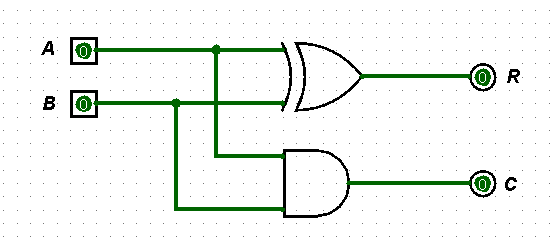
\includegraphics[width=10cm]{Somador/Circuito Meio-Somador.png}
    \caption{Circuito lógico do meio-somador.}
\label{fig:meio-somador}
\end{figure}

\subsection{Somador completo}
\label{subsec:somador_completo}

O \textbf{somador completo} é uma evolução do meio-somador.  
Além das duas entradas principais (\(A\) e \(B\)), ele também recebe um \textbf{Carry-In} — o transporte gerado pela soma anterior.  
Sua saída, por sua vez, produz o \textbf{Carry-Out}, que pode ser levado à próxima posição.

\begin{table}[H]
\centering
\begin{tabular}{|c|c|c|c|c|c|}
\hline
$C\textsc{in}$ & $A$ & $B$ & $C\textsc{out}$ & $R$ & Interpretação \\
\hline
0 & 0 & 0 & 0 & 0 & $0+0+0=00$ \\
0 & 0 & 1 & 0 & 1 & $0+0+1=01$ \\
0 & 1 & 0 & 0 & 1 & $0+1+0=01$ \\
0 & 1 & 1 & 1 & 0 & $0+1+1=10$ \\
1 & 0 & 0 & 0 & 1 & $1+0+0=01$ \\
1 & 0 & 1 & 1 & 0 & $1+0+1=10$ \\
1 & 1 & 0 & 1 & 0 & $1+1+0=10$ \\
1 & 1 & 1 & 1 & 1 & $1+1+1=11$ \\
\hline
\end{tabular}
\caption{Tabela-verdade do somador completo.}
\end{table}

A partir dessa tabela, é possível obter as seguintes expressões simplificadas (via Mapa de Karnaugh):

\[
C\textsc{out} = (A \cdot B) + (A \cdot C\textsc{in}) + (B \cdot C\textsc{in})
\]
\[
R = (A \oplus B) \oplus C\textsc{in}
\]

O circuito resultante é composto por dois meios-somadores e uma porta \textit{OR}, conforme mostra a Figura~\ref{fig:somador-completo}.

\begin{figure}[H]
\centering
    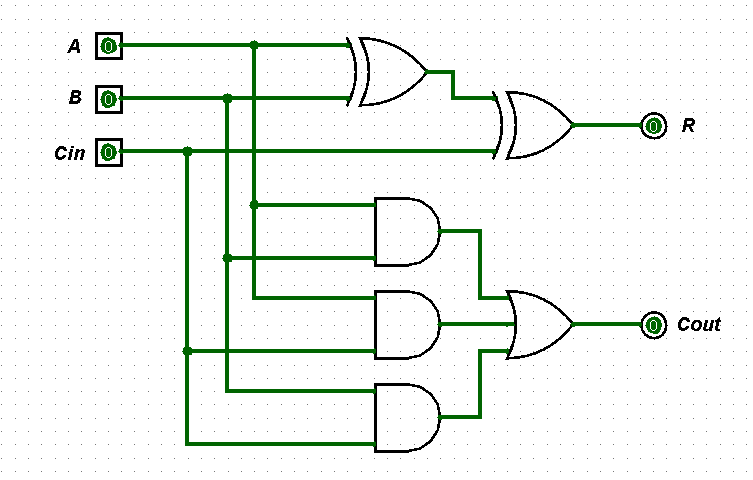
\includegraphics[width=10cm]{Somador/Circuito Somador Completo.png}
    \caption{Circuito lógico do somador completo.}
    \label{fig:somador-completo}
\hfill
\end{figure}

\subsection{Somador de n bits}

Por fim, ao conectar vários somadores completos em sequência, temos o \textbf{somador de n bits}.  
Nesse circuito, o transporte de saída (\textit{Carry-Out}) de cada estágio torna-se o \textit{Carry-In} do próximo, permitindo somar números binários com qualquer quantidade de bits.

\begin{figure}[H]
\centering
    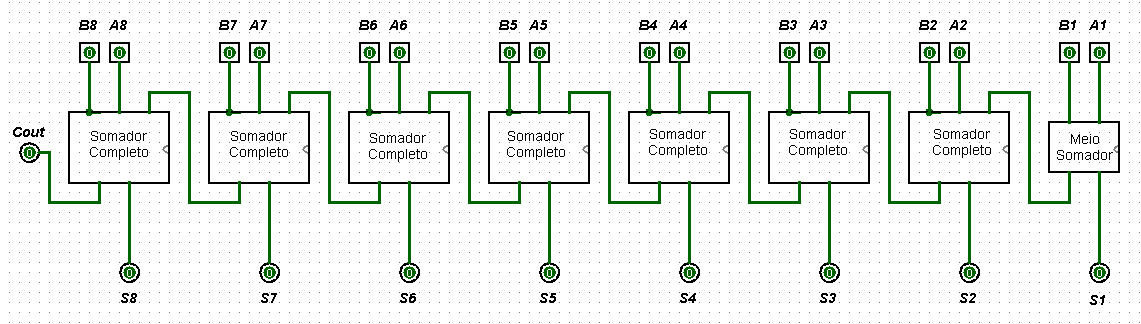
\includegraphics[width=\linewidth]{Somador/Circuito Somador.png}
    \caption*{Somador de 8 bits.}
\end{figure}

Cada saída representa um bit da soma final, e o último \textit{Carry-Out} indica se ocorreu um \textbf{overflow} — ou seja, se o resultado excedeu o tamanho máximo representável.

\begin{tcolorbox}[mynote, title=\textbf{Observação}]
A saída \textit{Carry-Out} pode também servir como entrada para outro bloco somador, permitindo construir somadores ainda maiores.  
Nesse caso, apenas o primeiro bloco da sequência precisa ser um meio-somador; os demais devem ser somadores completos.
\end{tcolorbox}

\subsection{Exercícios}

\begin{enumerate}
    \item Monte a tabela-verdade de um meio-somador e verifique as expressões das saídas \(C\) e \(R\).
    \item A partir do circuito do somador completo, determine o valor da soma quando \(A=1\), \(B=1\) e \(C_{in}=1\).
    \item Desenhe o esquema de um somador de 4 bits utilizando somadores completos em cascata.
    \item (Desafio) Explique como o mesmo circuito poderia realizar subtrações utilizando complemento de dois.
\end{enumerate}

\section{Subtrator}

O \textbf{subtrator} é um circuito lógico combinacional projetado para realizar a subtração entre números binários.  
Assim como o somador, ele é amplamente utilizado em processadores, calculadoras e sistemas digitais.  
Apesar de executar a operação inversa, sua estrutura lógica é bastante semelhante à do somador.

\subsection{Meio-subtrator}

Para compreender o funcionamento de um subtrator completo, é interessante começar com uma versão mais simples: o \textbf{meio-subtrator}.  

Ele recebe duas entradas — \(A\) (minuendo) e \(B\) (subtraendo) — e gera duas saídas:
\begin{itemize}
    \item \(R\): o \textbf{bit de diferença}, resultado de \(A - B\);
    \item \(B_o\): o \textbf{bit de empréstimo} (\textit{Borrow}), que indica quando é necessário “pedir emprestado” da próxima casa.
\end{itemize}

\begin{tcolorbox}[mynote, title=\textbf{\textit{Borrow}}]
O \textit{Borrow} é o equivalente ao famoso \textbf{"empresta 1"} da subtração.  
No sistema decimal, fazemos isso ao calcular $307 - 128$, por exemplo: emprestamos 1 da casa vizinha.  
No sistema binário, ocorre o mesmo — sempre que o minuendo é 0 e o subtraendo é 1, o circuito precisa “pedir emprestado”.
\end{tcolorbox}

A Tabela~\ref{tab:meio-subtrator} mostra as possíveis combinações das entradas e saídas:

\begin{table}[H]
\centering
\begin{tabular}{|c|c|c|c|c|}
\hline
$A$ & $B$ & $B_o$ & $R$ & Interpretação \\
\hline
0 & 0 & 0 & 0 & $0 - 0 = 0$ \\
0 & 1 & 1 & 1 & $0 - 1 = 1$ (com empréstimo) \\
1 & 0 & 0 & 1 & $1 - 0 = 1$ \\
1 & 1 & 0 & 0 & $1 - 1 = 0$ \\
\hline
\end{tabular}
\caption{Tabela-verdade do meio-subtrator.}
\label{tab:meio-subtrator}
\end{table}

A partir da tabela, obtemos as expressões booleanas das saídas:
\[
B_o = \overline{A} \cdot B \quad \text{e} \quad R = A \oplus B
\]

Essas expressões mostram que o circuito é formado por uma porta \textit{XOR} (para a diferença) e uma combinação \textit{NOT–AND} (para o empréstimo).

\begin{figure}[H]
\centering
    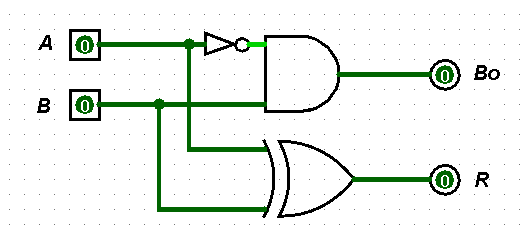
\includegraphics[width=10cm]{Subtrator/Circuito Meio-Subtrator.png}
    \caption*{Circuito lógico do meio-subtrator.}
\end{figure}

\subsection{Subtrator completo}

O \textbf{subtrator completo} é uma extensão do meio-subtrator que considera também o \textit{empréstimo de entrada} (\(B_{in}\)), vindo da subtração anterior.  
Assim, ele possui três entradas — \(A\), \(B\) e \(B_{in}\) — e duas saídas:
\begin{itemize}
    \item \(R\): diferença resultante;
    \item \(B_o\): empréstimo de saída.
\end{itemize}

\begin{table}[H]
\centering
\begin{tabular}{|c|c|c|c|c|c|}
\hline
$A$ & $B$ & $B_{in}$ & $R$ & $B_o$ & Interpretação \\
\hline
0 & 0 & 0 & 0 & 0 & $0-0-0=0$ \\
0 & 0 & 1 & 1 & 1 & $0-0-1=1$ (com empréstimo) \\
0 & 1 & 0 & 1 & 1 & $0-1-0=1$ (com empréstimo) \\
0 & 1 & 1 & 0 & 1 & $0-1-1=0$ (com empréstimo) \\
1 & 0 & 0 & 1 & 0 & $1-0-0=1$ \\
1 & 0 & 1 & 0 & 0 & $1-0-1=0$ \\
1 & 1 & 0 & 0 & 0 & $1-1-0=0$ \\
1 & 1 & 1 & 1 & 1 & $1-1-1=1$ (com empréstimo) \\
\hline
\end{tabular}
\caption{Tabela-verdade do subtrator completo.}
\label{tab:subtrator-completo}
\end{table}

Com base na tabela e na simplificação via Mapa de Karnaugh, temos:
\[
B_o = \overline{A}B + \overline{A}B_{in} + B B_{in} \quad \text{e} \quad R = A \oplus B \oplus B_{in}
\]

O circuito pode ser construído conectando dois meios-subtratores e uma porta \textit{OR}, como mostrado na Figura~\ref{fig:subtrator-completo}.

\begin{figure}[H]
\centering
    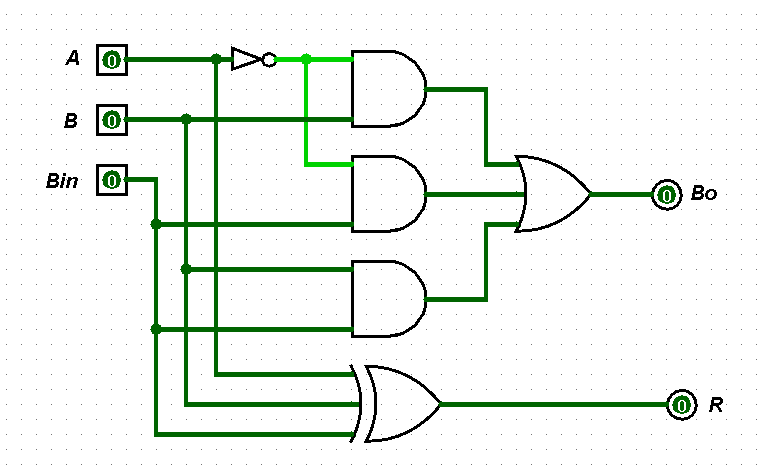
\includegraphics[width=10cm]{Subtrator/Circuito Subtrator Completo.png}
    \caption{Circuito lógico do subtrator completo.}
\label{fig:subtrator-completo}
\end{figure}

\subsection{Subtrator de n bits}

Da mesma forma que no somador, é possível criar subtratores com vários bits conectando múltiplos subtratores completos em sequência.  
O \textit{Borrow-Out} de cada estágio torna-se o \textit{Borrow-In} do estágio seguinte.

\begin{figure}[H]
\centering
    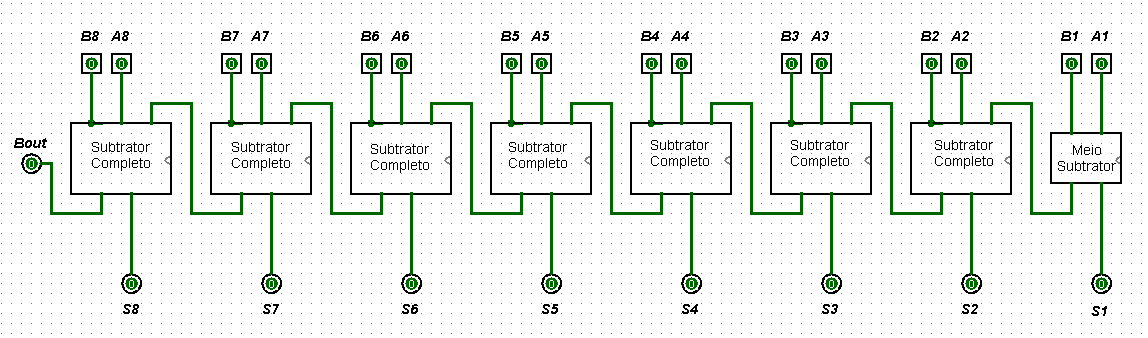
\includegraphics[width=\linewidth]{Subtrator/Circuito Subtrator.png}
    \caption{Circuito subtrator de 8 bits.}
\end{figure}

Assim, cada saída representa um bit da diferença final, e o último \textit{Borrow-Out} indica se foi necessário um empréstimo além do tamanho representável (ou seja, se a subtração “estourou” o limite de bits).

\subsection{Implementação alternativa}

Também é possível implementar a subtração utilizando apenas o circuito somador.  
Isso porque, no mundo binário, subtrair um número é equivalente a somar o seu \textbf{complemento de dois}:

\[
A - B = A + (-B) = A + (\overline{B} + 1)
\]

Para isso:
\begin{itemize}
    \item Inverte-se o subtraendo \(B\) com portas \textit{NOT};
    \item Define-se o primeiro \textit{Carry-In} do somador como 1, representando a adição do “+1” do complemento de dois.
\end{itemize}

Essa abordagem é amplamente usada em processadores reais, já que elimina a necessidade de dois circuitos distintos para soma e subtração.  
Um mesmo somador pode realizar ambas as operações, dependendo apenas do controle do sinal que inverte os bits de \(B\).

\begin{figure}[H]
\centering
    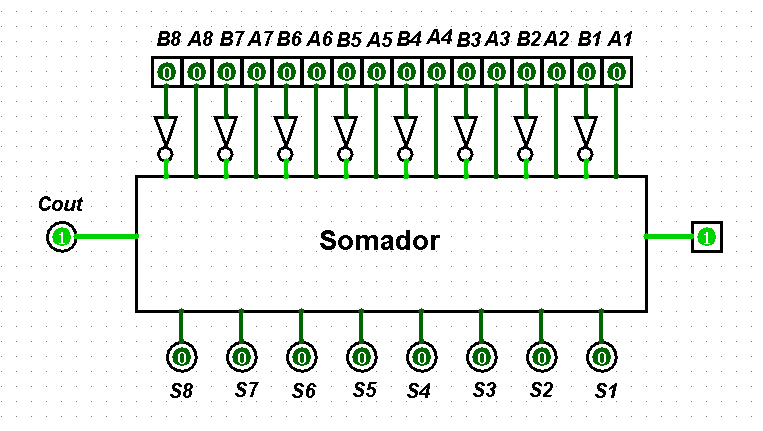
\includegraphics[width=13cm]{Subtrator/Subtrator Alternativo.png}
    \caption*{Circuito subtrator de 8 bits alternativo.}
\end{figure}

\begin{tcolorbox}[mynote, title=\textbf{Observação}]
O uso do complemento de dois é o método mais prático e eficiente para realizar subtrações em sistemas digitais.  
Assim, o mesmo circuito de soma pode operar como subtrator apenas ajustando um único sinal lógico.
\end{tcolorbox}

\subsection{Exercícios}

\begin{enumerate}
    \item Elabore a tabela-verdade do meio-subtrator e derive as expressões para \(R\) e \(B_o\).
    \item Determine o resultado da operação binária \(1010 - 0111\) utilizando um subtrator de 4 bits.
    \item Simule mentalmente o comportamento do subtrator completo para \(A=0\), \(B=1\) e \(B_{in}=1\).
    \item (Desafio) Explique como a subtração pode ser implementada com um circuito somador usando o complemento de dois.
\end{enumerate}

\section{Multiplicador}

O \textbf{multiplicador} é um circuito combinacional formado por portas lógicas e caixas-pretas que realiza multiplicações entre números binários.  
Ele é um dos blocos mais importantes de uma \textit{Unidade Lógica e Aritmética (ULA)}, sendo amplamente utilizado em processadores, DSPs e outros sistemas digitais.  

Apesar de parecer complexo, o multiplicador nada mais é do que uma versão organizada do processo manual de multiplicação — aquele mesmo método em que repetimos somas deslocadas, linha por linha.  

Existem duas formas principais de implementar um multiplicador:

\begin{itemize}
    \item \textbf{Por tabela-verdade:} listando todas as combinações possíveis entre as entradas e suas saídas correspondentes;
    \item \textbf{Por lógica combinacional:} aplicando o raciocínio de multiplicações parciais e somas sucessivas, semelhante à multiplicação no papel.
\end{itemize}

A seguir, exploraremos ambas as abordagens.

---

\subsection{Multiplicador por tabela-verdade}

Um multiplicador baseado em tabela-verdade funciona da mesma forma que qualquer circuito combinacional:  
são listadas todas as possíveis combinações das entradas e as respectivas saídas do resultado da multiplicação.

Como exemplo, construiremos um multiplicador de $2 \times 2$ bits.

\begin{tcolorbox}[mynote, title=\textbf{Lembre-se: número de bits da saída}]
A quantidade de bits do resultado é sempre a soma dos bits das entradas.  
Assim, um multiplicador de 2 bits por 2 bits gera uma saída de 4 bits.
\end{tcolorbox}

A Tabela~\ref{tab:multiplicador-2x2} mostra todas as combinações de entradas e suas saídas correspondentes:

\begin{table}[h] 
\centering 
\begin{tabular}{|c c|c c|c c c c|c|} 
\hline 
\multicolumn{2}{|c|}{\textbf{A}} & \multicolumn{2}{c|}{\textbf{B}} & \multicolumn{4}{c|}{\textbf{Resultado}} & \textbf{Interpretação} \\ 
\hline 
$A_1$ & $A_0$ & $B_1$ & $B_0$ & $R_3$ & $R_2$ & $R_1$ & $R_0$ & \\
\hline 
0 & 0 & 0 & 0 & 0 & 0 & 0 & 0 & $0 \times 0 = 0$ \\ 
0 & 0 & 0 & 1 & 0 & 0 & 0 & 0 & $0 \times 1 = 0$ \\ 
0 & 0 & 1 & 0 & 0 & 0 & 0 & 0 & $0 \times 2 = 0$ \\ 
0 & 0 & 1 & 1 & 0 & 0 & 0 & 0 & $0 \times 3 = 0$ \\ 
0 & 1 & 0 & 0 & 0 & 0 & 0 & 0 & $1 \times 0 = 0$ \\ 
0 & 1 & 0 & 1 & 0 & 0 & 0 & 1 & $1 \times 1 = 1$ \\ 
0 & 1 & 1 & 0 & 0 & 0 & 1 & 0 & $1 \times 2 = 2$ \\ 
0 & 1 & 1 & 1 & 0 & 0 & 1 & 1 & $1 \times 3 = 3$ \\ 
1 & 0 & 0 & 0 & 0 & 0 & 0 & 0 & $2 \times 0 = 0$ \\ 
1 & 0 & 0 & 1 & 0 & 0 & 1 & 0 & $2 \times 1 = 2$ \\ 
1 & 0 & 1 & 0 & 0 & 1 & 0 & 0 & $2 \times 2 = 4$ \\ 
1 & 0 & 1 & 1 & 0 & 1 & 1 & 0 & $2 \times 3 = 6$ \\ 
1 & 1 & 0 & 0 & 0 & 0 & 0 & 0 & $3 \times 0 = 0$ \\ 
1 & 1 & 0 & 1 & 0 & 0 & 1 & 1 & $3 \times 1 = 3$ \\ 
1 & 1 & 1 & 0 & 0 & 1 & 1 & 0 & $3 \times 2 = 6$ \\ 
1 & 1 & 1 & 1 & 1 & 0 & 0 & 1 & $3 \times 3 = 9$ \\
\hline
\end{tabular}
\caption{Tabela-verdade resumida para o multiplicador de $2 \times 2$ bits.}
\label{tab:multiplicador-2x2}
\end{table}

A partir da simplificação das saídas (via Mapa de Karnaugh ou observação direta), temos:

\[ R_0 = A_0 \cdot B_0 \] 
\[ R_1 = (A_1 \cdot A_0 \cdot \overline{B_1} \cdot B_0) + (\overline{A_1} \cdot A_0 \cdot B_1) + (A_0 \cdot B_1 \cdot \overline{B_0}) + (A_1 \cdot \overline{A_0} \cdot B_1)\]
\[ R_2 = (A_1 \cdot \overline{A_0} \cdot B_1) + (A_1 \cdot B_1 \cdot \overline{B_0})\]
\[ R_3 = A_1 \cdot A_0 \cdot B_1 \cdot B_0 \]

Essas expressões podem ser traduzidas em um circuito combinacional, composto basicamente por portas AND (para gerar os produtos parciais) e portas OR (para somá-los).

\begin{figure}[H]
\centering
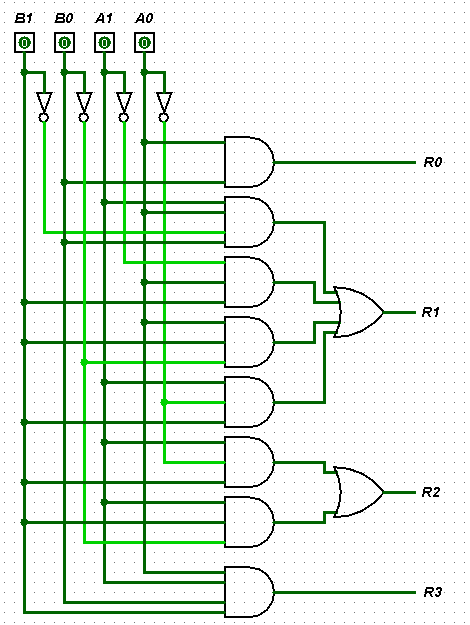
\includegraphics[width=8cm]{Multiplicador/Multiplicador Alternativo.png}
\caption{Circuito lógico de um multiplicador de $2 \times 2$ bits.}
\label{fig:multiplicador-2x2}
\end{figure}

\begin{tcolorbox}[mynote, title=\textbf{Generalização}]
O mesmo raciocínio pode ser aplicado a qualquer multiplicador de $n \times m$ bits.  
O circuito cresce proporcionalmente ao número de bits das entradas — quanto maior o tamanho dos operandos, maior o número de portas e somadores necessários.
\end{tcolorbox}

---

\subsection{Multiplicador combinacional}

O \textbf{multiplicador combinacional} aplica diretamente a lógica da multiplicação no papel — só que feita com portas lógicas.

Cada bit do multiplicador (\(B\)) é conectado a todas as entradas do multiplicando (\(A\)) por meio de portas \textit{AND}.  
Essas combinações geram os chamados \textbf{produtos parciais}, que depois são \textbf{somados} de forma deslocada, assim como fazemos manualmente ao multiplicar dois números decimais.

\begin{center}
\begin{tabular}{c c c c}
  &  & $A_1$ & $A_0$ \\
  & $\times$ & $B_1$ & $B_0$ \\
\hline
  &  & $A_1B_0$ & $A_0B_0$ \\
  & $A_1B_1$ & $A_0B_1$ & + \\
\hline
$R_3$ & $R_2$ & $R_1$ & $R_0$
\end{tabular}
\end{center}

\vspace{0.1cm}

O primeiro produto parcial é escrito normalmente;  
os seguintes são \textbf{deslocados uma posição à esquerda} — isso representa o aumento do valor posicional dos bits (de unidades para dezenas, centenas, etc., no sistema binário).

Esses produtos parciais são então somados por meio de somadores completos, formando uma estrutura de \textbf{array} (ou matriz de somadores).  
O resultado final tem $n + m$ bits.

\begin{figure}[H]
\centering
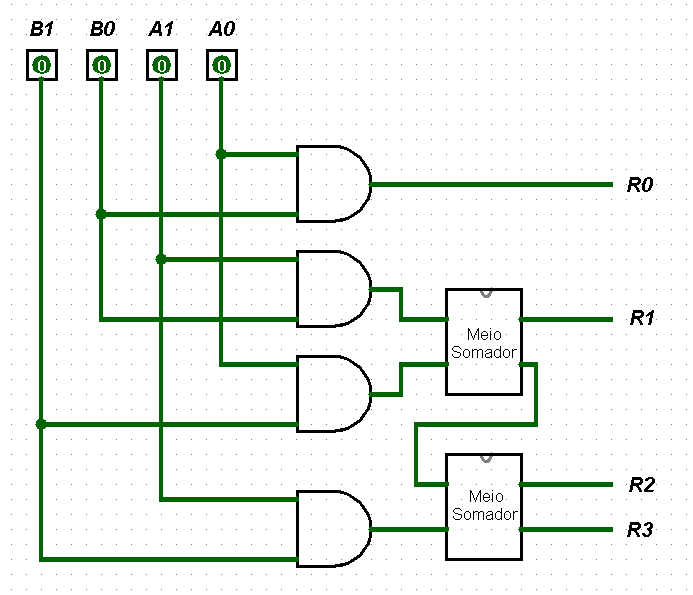
\includegraphics[width=13cm]{Multiplicador/Multiplicador Combinacional.png}
\caption{Estrutura de um multiplicador combinacional de $2 \times 2$ bits.}
\label{fig:multiplicador-combinacional}
\end{figure}

\begin{tcolorbox}[mynote, title=\textbf{Multiplicadores maiores}]
A estrutura combinacional pode ser expandida para qualquer número de bits.  
Para operandos maiores, o circuito se organiza em camadas diagonais de somadores — formando um padrão conhecido como \textbf{array multiplier}.
\end{tcolorbox}

---

\subsection{Conclusão}

O multiplicador é, essencialmente, uma combinação de \textbf{portas AND} (para gerar produtos parciais) e \textbf{somadores} (para somá-los).  
A versão por tabela-verdade é conceitualmente útil para pequenos números de bits, mas se torna inviável em circuitos grandes.  
Já o método combinacional é o mais prático e escalável, sendo o preferido em sistemas reais.

\begin{tcolorbox}[mynote, title=\textbf{Resumo do funcionamento}]
Cada linha do multiplicador representa uma soma condicional:  
se o bit do multiplicador for 1, somamos o multiplicando deslocado; se for 0, nada é somado.  
O circuito faz isso automaticamente, multiplicando por meio de repetições de soma e deslocamento.
\end{tcolorbox}

\subsection{Exercícios}

\begin{enumerate}
    \item Construa a tabela-verdade para um multiplicador de \(1 \times 2\) bits.
    \item Determine o resultado da multiplicação \(10_2 \times 11_2\) utilizando o raciocínio dos produtos parciais.
    \item Explique o papel das portas AND e dos somadores no funcionamento do multiplicador combinacional.
    \item (Desafio) Proponha uma forma de otimizar um multiplicador de 4 bits, reduzindo o número de somadores necessários.
\end{enumerate}

\section{Decodificadores e Codificadores}

Até este ponto, trabalhamos com circuitos que operam diretamente sobre valores binários.  
Entretanto, em sistemas digitais reais, é comum a interação com informações representadas de forma simbólica, como números decimais, caracteres e sinais provenientes de teclados ou \textit{displays}.  

Para que haja uma comunicação eficaz entre o mundo físico e o digital, é necessário realizar uma conversão entre representações simbólicas e códigos binários.  
Essa função é desempenhada por dois circuitos combinacionais fundamentais: os \textbf{decodificadores} e os \textbf{codificadores}.  

\begin{itemize}
    \item \textbf{Codificador:} converte um sinal simbólico em uma representação binária.
    \item \textbf{Decodificador:} realiza o processo inverso, convertendo um código binário em uma saída simbólica.
\end{itemize}

---

\subsection{Decodificador}

O \textbf{decodificador} é um circuito combinacional cuja função é identificar uma combinação binária de entrada e ativar a respectiva saída correspondente.  
Em termos práticos, ele “traduz” um código binário em uma única linha de saída ativa.  

Por exemplo, um \textbf{decodificador 2$\rightarrow$4} possui duas entradas binárias ($E_1$ e $E_0$) e quatro saídas ($S_0$, $S_1$, $S_2$, $S_3$).  
Cada combinação das entradas ativa exclusivamente uma das saídas, conforme apresentado na Tabela~\ref{tab:decodificador2x4}.

\begin{table}[H]
\centering
\renewcommand{\arraystretch}{1.2}
\begin{tabular}{|c|c|c|}
\hline
$E_1$ & $E_0$ & Saída ativa \\ 
\hline
0 & 0 & $S_0$ \\
0 & 1 & $S_1$ \\
1 & 0 & $S_2$ \\
1 & 1 & $S_3$ \\
\hline
\end{tabular}
\caption{Tabela-verdade de um decodificador 2$\rightarrow$4.}
\label{tab:decodificador2x4}
\end{table}

As expressões lógicas de cada saída são obtidas diretamente da tabela-verdade:

\[
S_0 = \overline{E_1} \cdot \overline{E_0}, \quad
S_1 = \overline{E_1} \cdot E_0, \quad
S_2 = E_1 \cdot \overline{E_0}, \quad
S_3 = E_1 \cdot E_0.
\]

Essas expressões podem ser implementadas por meio de portas lógicas \textit{AND} e \textit{NOT}, resultando em um circuito de estrutura simples e direta.

\begin{figure}[H]
\centering
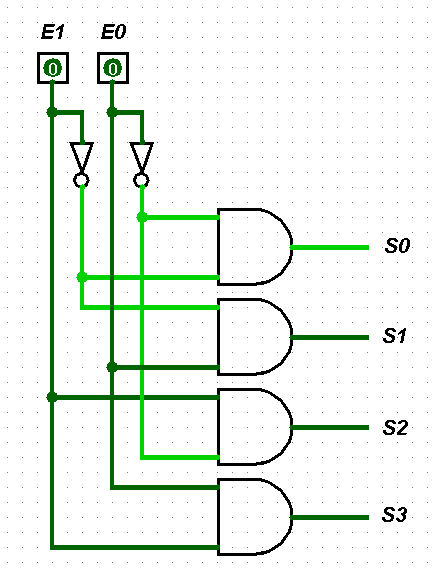
\includegraphics[width=8cm]{Deco-Codificador/Circuito Decodificador.png}
\caption{Circuito lógico de um decodificador 2$\rightarrow$4.}
\end{figure}

\begin{tcolorbox}[mynote, title=\textbf{Aplicações práticas}]
Os decodificadores são amplamente utilizados em:
\begin{itemize}
    \item Seleção de endereços de memória (ativação de uma linha específica);
    \item Controle de \textit{displays} de sete segmentos e painéis indicadores;
    \item Seleção de registradores e dispositivos em sistemas microprocessados.
\end{itemize}
\end{tcolorbox}

---

\subsection{Codificador}

O \textbf{codificador} executa a operação inversa ao decodificador.  
Ele recebe múltiplas entradas — das quais apenas uma está ativa — e gera um código binário correspondente à linha de entrada ativada.  

Por exemplo, um \textbf{codificador 4$\rightarrow$2} possui quatro entradas ($E_3$, $E_2$, $E_1$, $E_0$) e duas saídas ($S_1$, $S_0$).  
A Tabela~\ref{tab:codificador4x2} apresenta o funcionamento deste circuito.

\begin{table}[H]
\centering
\renewcommand{\arraystretch}{1.2}
\begin{tabular}{|c|c|c|}
\hline
Entrada ativa & $S_1$ & $S_0$ \\
\hline
$E_0$ & 0 & 0 \\
$E_1$ & 0 & 1 \\
$E_2$ & 1 & 0 \\
$E_3$ & 1 & 1 \\
\hline
\end{tabular}
\caption{Tabela-verdade de um codificador 4$\rightarrow$2.}
\label{tab:codificador4x2}
\end{table}

As expressões lógicas das saídas são:

\[
S_0 = E_1 + E_3, \quad S_1 = E_2 + E_3.
\]

Essas funções podem ser implementadas utilizando apenas portas \textit{OR}, tornando o circuito compacto e eficiente.

\begin{figure}[H]
\centering
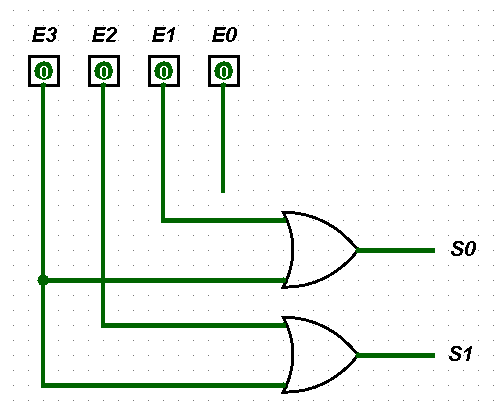
\includegraphics[width=10cm]{Deco-Codificador/Circuito Codificador.png}
\caption{Circuito lógico de um codificador 4$\rightarrow$2.}
\end{figure}

\begin{tcolorbox}[mynote, title=\textbf{Codificador com prioridade}]
Na prática, pode ocorrer que mais de uma entrada esteja ativa simultaneamente.  
Nesses casos, utiliza-se o \textbf{codificador com prioridade}, que considera válida apenas a entrada de maior ordem (ou de maior peso binário), garantindo a consistência do resultado.
\end{tcolorbox}

\begin{tcolorbox}[mynote, title=\textbf{Aplicações práticas}]
Os codificadores são frequentemente empregados em:
\begin{itemize}
    \item Teclados e painéis de controle, convertendo teclas em códigos binários;
    \item Sistemas de interrupção, determinando a prioridade entre múltiplas solicitações;
    \item Conversores de sinais provenientes de sensores e chaves seletoras.
\end{itemize}
\end{tcolorbox}

---

\subsection{Associação entre Codificadores e Decodificadores}

Em diversos sistemas digitais, os codificadores e decodificadores atuam de forma complementar.  
Enquanto o codificador converte um sinal físico em código binário, o decodificador interpreta esse código e o converte novamente em uma forma simbólica ou de controle.  

Um exemplo clássico ocorre em teclados e \textit{displays} numéricos.  
Ao pressionar a tecla “2”, o circuito codificador gera o código binário 0010, o qual é então enviado ao decodificador.  
Este, por sua vez, ativa os segmentos correspondentes no \textit{display}, exibindo o número “2”.

\begin{center}
\textbf{[Tecla “2” pressionada]} $\Rightarrow$ (codificador) $\Rightarrow$ 0010 $\Rightarrow$ (decodificador) $\Rightarrow$ Exibição no \textit{display}.
\end{center}

\begin{tcolorbox}[mynote, title=\textbf{Resumo conceitual}]
\begin{itemize}
    \item O \textbf{codificador} realiza a \textit{compactação da informação}, transformando sinais físicos em representações binárias;
    \item O \textbf{decodificador} realiza a \textit{expansão da informação}, convertendo códigos binários em ações ou sinais específicos;
    \item Juntos, constituem a base da comunicação entre o ambiente físico e o domínio lógico-digital.
\end{itemize}
\end{tcolorbox}

\subsection{Exercícios}

\begin{enumerate}
    \item Construa a tabela-verdade de um decodificador \(3 \rightarrow 8\).
    \item A partir de um codificador \(8 \rightarrow 3\), determine a saída binária quando a entrada ativa for a linha 5.
    \item Explique o funcionamento de um codificador com prioridade e cite uma aplicação real.
    \item (Desafio) Desenhe um circuito em que um codificador e um decodificador trabalhem em conjunto para representar um teclado e um \textit{display} numérico.
\end{enumerate}

\section{Circuito Combinacional}

\textbf{Circuitos combinacionais} são aqueles que só dependem do estado atual da entrada, ou seja, não possuem \textbf{memória}.
Um exemplo simples é um circuito onde a saída $f$ é dada por $f = A \cdot B$, usando uma porta \textbf{AND} de duas entradas.

\vspace{0.5cm}

Esses circuitos incluem:

\begin{itemize}
   \item Somadores
   \item Comparadores
   \item Codificadores
   \item Decodificadores
   \item Multiplexadores
\end{itemize}

\section{Circuitos Sequenciais}

\textbf{Diferente} dos circuitos combinacionais, os \textbf{circuitos sequenciais} dependem tanto das \textbf{entradas atuais} como do \textbf{estado anterior (memória)}.

Eles utilizam elementos de \textbf{armazenamento}, como flip-flops, para guardar o estado interno. Portanto, a saída é uma função das entradas e do estado armazenado. 

\vspace{0.5cm}

São utilizados em:

\begin{itemize}
   \item Regustradores
   \item Máquinas de Estados
   \item Contadores
\end{itemize}

\vspace{0.5cm}

Os circuitos sequenciais podem ser \textbf{síncronos} (controlados por um sinal de clock) ou \textbf{assíncronos} (controlados por variações nas entradas)

\section{Multiplexadores e Demultiplexadores}

\subsection{MUX}
    
O Multiplexador (MUX) é um \textbf{circuito lógico combinacional} que seleciona uma entre X entradas de dados e a envia para uma única saída, conforme os Y sinais de controle.
\textbf{Normalmente usamos a relação X = $2^Y$} 
    
Em outras palavras, ele atua como um "canal seletor":
    
Várias entradas → 1 saída escolhida.

\begin{tcolorbox}[mynote, title=\textbf{Exemplo}]
Pensando em algo cotidiano: imagine um chuveiro elétrico com diferentes opções de temperatura, em que cada opção é uma entrada ($X_0, X_1, X_2, X_3$). O botão do chuveiro é a entrada de seleção e a água que sai é a saída. Ao escolher uma posição no botão, apenas uma entrada é conectada à saída. O MUX faz exatamente isso, só que de forma digital e automática,
controlada por bits.
\end{tcolorbox}

\subsubsection{MUX 4x1}

\begin{figure}[h]
\centering
\begin{tikzpicture}[scale=1]

% Corpo
\draw (0,0) -- (0,4) -- (2,3) -- (2,1) -- cycle;

% Entradas
\draw (-1,3.5) -- (0,3.5) node[midway,above] {$X_0$};
\draw (-1,2.5) -- (0,2.5) node[midway,above] {$X_1$};
\draw (-1,1.5) -- (0,1.5) node[midway,below] {$X_2$};
\draw (-1,0.5) -- (0,0.5) node[midway,below] {$X_3$};

% Saída
\draw (2,2) -- (3,2) node[right] {$S$};

% Seletores
\draw (0.8,-1) -- (0.8,0) node[midway,left] {$Y_1$};
\draw (1.2,-1) -- (1.2,0) node[midway,right] {$Y_0$};

% Rótulo interno
\node at (1,2) {MUX};

\end{tikzpicture}
\end{figure}

Um MUX com 4 entradas binárias ($X_0, X_1, X_2, X_3$), 2 sinais de controle ($Y_0, Y_1$) e 1 saída ($S$), também denominado de multiplexador 4x1, é definido pela tabela verdade:
\begin{table}[h]
\centering

{\large
\begin{tabular}{|c|c|c|}
\hline
$S_1$ & $S_0$ & $Y$ \\ \hline
0 & 0 & $D_0$ \\ \hline
0 & 1 & $D_1$ \\ \hline
1 & 0 & $D_2$ \\ \hline
1 & 1 & $D_3$ \\ \hline
\end{tabular}
}

\caption{Tabela verdade do multiplexador 4x1}
\label{tab:mux4x1}
\end{table}

\subsection{DEMUX}
O Demultiplexador (DEMUX) é um \textbf{circuito lógico combinacional} que recebe \textbf{uma única entrada de dados} e a direciona para \textbf{uma entre X saídas}, conforme os Y sinais de controle.
\textbf{Normalmente usamos a relação X = $2^Y$}

Em outras palavras, ele atua como um distribuidor de dados:

1 entrada → várias saídas (apenas uma ativa por vez).

\begin{tcolorbox}[mynote, title=\textbf{Exemplo}]
Imagine um centro de distribuição dos Correios.

A encomenda que chega representa a \textbf{entrada única} do DEMUX.  
As diferentes rotas de entrega (bairros ou cidades) representam as \textbf{saídas} ($S_0, S_1, S_2, S_3$).  
O CEP da encomenda funciona como o \textbf{sinal de controle}.

De acordo com esse código, a encomenda é enviada para \textbf{apenas uma rota específica}, enquanto as demais não recebem nada naquele momento.
O DEMUX funciona exatamente assim: ele recebe um único dado e o direciona para uma única saída, conforme os bits de seleção.
\end{tcolorbox}

\subsubsection{DEMUX 1x4}

\begin{figure}[h]
\centering
\begin{tikzpicture}[scale=1]

\draw (0,1) -- (0,3) -- (2,4) -- (2,0) -- cycle;

\draw (-1,2) -- (0,2) node[midway,above] {$X$};

\draw (2,3.5) -- (3,3.5) node[right] {$S_0$};
\draw (2,2.5) -- (3,2.5) node[right] {$S_1$};
\draw (2,1.5) -- (3,1.5) node[right] {$S_2$};
\draw (2,0.5) -- (3,0.5) node[right] {$S_3$};

\draw (0.8,0) -- (0.8,-1) node[midway,left] {$Y_1$};
\draw (1.2,0) -- (1.2,-1) node[midway,right] {$Y_0$};

\node at (1,2) {DEMUX};

\end{tikzpicture}
\end{figure}

Um DEMUX com 1 entrada binária ($D$), 2 sinais de controle ($S_0, S_1$) e 4 saídas ($Y_0, Y_1, Y_2, Y_3$), também denominado de demultiplexador 1x4, é definido pela tabela verdade:

\begin{table}[h]
\centering

\begin{tabular}{|c|c|c|}
\hline
$Y_1$ & $Y_0$ & Saída ativa \\ \hline
0 & 0 & $S_0 = X$ \\ \hline
0 & 1 & $S_1 = X$ \\ \hline
1 & 0 & $S_2 = X$ \\ \hline
1 & 1 & $S_3 = X$ \\ \hline
\end{tabular}

\caption{Tabela verdade do demultiplexador 1x4}
\label{tab:demux4x1}
\end{table}

\newpage
\subsection{Multiplexador x Demultiplexador}

\begin{table}[h]
\centering
\begin{tabular}{|l|c|c|}
\hline
\textbf{Característica} & \textbf{MUX} & \textbf{DEMUX} \\ \hline
Tipo de circuito & Combinacional & Combinacional \\ \hline
Entradas de dados & Várias & Uma \\ \hline
Entradas de seleção & $m$ bits & $m$ bits \\ \hline
Saídas & Uma & Várias \\ \hline
Função principal & Selecionar entrada & Direcionar saída \\ \hline
Fluxo de dados & Entradas $\rightarrow$ saída única & Entrada única $\rightarrow$ saídas \\ \hline
\end{tabular}
\caption{Comparação entre MUX e DEMUX}
\end{table}

\begin{figure}[h]
\centering
\begin{tikzpicture}[>=latex]

\node (x0) at (0,1.8) [draw, rectangle, minimum width=2.6cm, minimum height=0.9cm] {$X_0$ (Frio)};
\node (x1) at (0,0.6) [draw, rectangle, minimum width=2.6cm, minimum height=0.9cm] {$X_1$ (Ambient)};
\node (x2) at (0,-0.6) [draw, rectangle, minimum width=2.6cm, minimum height=0.9cm] {$X_2$ (Quente)};
\node (x3) at (0,-1.8) [draw, rectangle, minimum width=2.6cm, minimum height=0.9cm] {$X_3$ (Muito quente)};

\node (mux) at (4,0) [draw, rectangle, minimum width=3cm, minimum height=3.8cm] {MUX};

\node (out) at (8,0) [draw, rectangle, minimum width=2.6cm, minimum height=1.4cm]{Água do chuveiro};

% Setas
\draw[->] (x0) -- (mux);
\draw[->] (x1) -- (mux);
\draw[->] (x2) -- (mux);
\draw[->] (x3) -- (mux);
\draw[->] (mux) -- node[above] {$Y$} (out);

\node (sel) at (4,-3) {Botão do chuveiro (seleção $S_1S_0$)};
\draw[->] (sel) -- (mux);

\end{tikzpicture}
\caption{Exemplo de um MUX usando o seletor de temperatura do chuveiro}
\end{figure}

\begin{figure}[h]
\centering
\begin{tikzpicture}[>=latex, node distance=2cm, every node/.style={align=center}]

\node (entrada) [draw, rectangle, minimum width=2.5cm, minimum height=1cm] {Carta};

\node (demux) [draw, rectangle, right=2cm of entrada, minimum width=3cm, minimum height=3cm] {DEMUX \\ (Correios)};

\node (saida1) [draw, rectangle, right=2.5cm of demux, yshift=1.2cm] {Bairro A};
\node (saida2) [draw, rectangle, right=2.5cm of demux] {Bairro B};
\node (saida3) [draw, rectangle, right=2.5cm of demux, yshift=-1.2cm] {Bairro C};

\draw[->] (entrada) -- (demux);
\draw[->] (demux) -- (saida1);
\draw[->] (demux) -- (saida2);
\draw[->] (demux) -- (saida3);

\node (sel) [below=1.5cm of demux] {Seleção (CEP)};
\draw[->] (sel) -- (demux);

\end{tikzpicture}
\caption{Exemplo de funcionamento de um DEMUX usando a analogia dos correios}
\end{figure}

%------------------------------------------------------
\newpage
\section{Unidade Lógica Aritmética (ULA)}
A Unidade Lógica Aritmética (ULA) tem como função realizar operações aritméticas e lógicas sobre dados binários,
como soma, subtração, comparação e operações lógicas básicas.


A ULA recebe como entrada dois operandos binários, além de sinais de controle que definem qual operaçãodeve ser executada.
O resultado da operação é disponibilizado na saída e pode ser armazenado ou utilizado por outros blocos do sistema.

\begin{figure}[h]
\centering

\begin{tikzpicture}[line cap=round,line join=round, scale=1.2]
\tikzset{arr/.style={-Latex, line width=0.9pt}}

\draw[line width=0.9pt]
  (-2,0) -- (-0.35,0) -- (0,-0.28) -- (0.35,0) -- (2,0) -- (1.1,-1.25) -- (-1.3,-1.25) -- cycle;

\node at (-0.95,-0.25) {\large A};
\node at ( 0.95,-0.25) {\large B};
\node at (-1.55,-0.55) {\large C};
\node at ( 0.00,-0.95) {\large S};

\draw[arr] (-0.95,1.1) -- (-0.95,0);

\draw[arr] ( 0.95,1.1) -- ( 0.95,0);

\draw[arr] (-3,-0.55) -- (-2,-0.55);

\draw[arr] (0,-1.25) -- (0,-2.05);

\end{tikzpicture}

\caption{Unidade Lógica e Aritmética}
\label{fig:ula}
\end{figure}


Na imagem a operação realizada pela ULA que conta com as entradas A e B, é determinada por um sinal de controle C e o resultado é obtido na saída S.

As operações executadas pela ULA podem ser classificadas em dois grupos principais: 
\begin{itemize}
\item operações aritméticas.
\item operações lógicas.
\end{itemize}

Entre as operações aritméticas mais comuns estão a soma e a subtração.
Já as operações lógicas incluem AND, OR, XOR e NOT.
A seleção da operação é feita por sinais de controle, normalmente representados por bits.

\begin{tcolorbox}[mynote, title=\textbf{Exemplo}]
Vamos realizar a soma entre os números 8 e 6.

\begin{center}
\begin{tikzpicture}[
    line cap=round,
    line join=round,
    scale=0.75,
    transform shape
]
\tikzset{arr/.style={-Latex, line width=0.9pt}}

\draw[line width=0.9pt] (-2.2,0) -- (-0.6,0) -- (0,-0.4) -- (0.6,0) -- (2.2,0) -- (1.3,-1.4) -- (-1.5,-1.4) -- cycle;

\node at (-1.0,-0.3) {\normalsize 8};
\node at ( 1.0,-0.3) {\normalsize 6};
\node at ( 0.0,-0.9) {\normalsize 14};

\draw[arr] (-1.0,0.9) -- (-1.0,0.05);
\draw[arr] ( 1.0,0.9) -- ( 1.0,0.05);

\draw[arr] (-3.0,-0.6) -- (-2.22,-0.6);
\node[above] at (-2.6,-0.6) {\normalsize Soma};

\draw[arr] (0,-1.4) -- (0,-2.0);

\end{tikzpicture}

\captionsetup{hypcap=false}
\captionof{figure}{Soma na ULA: $8 + 6 = 14$}
\label{fig:ula-soma}
\end{center}


\end{tcolorbox}

%------------------------------------------------------
\newpage
\section{Formas de onda}

Em um computador, toda a informação é processada com base nos \textbf{sinais elétricos} que passam pelos seus circuitos. Nesse contexto, existem dois tipos de interpretações de sinais elétricos: analógica e digital.

\begin{multicols}{2}
\raggedcolumns
\begin{itemize}
   \item \textbf{Sinais analógicos}: variam continuamente no tempo, podendo atingir qualquer valor dentro de um intervalo de tensão.
   \item \textbf{Sinais digitais}: variam de forma descontínua ou discreta, isto é, saltam entre valores específicos e pré-definidos. Quando os analisamos, não nos preocupamos com os valores intermediários a eles.
\end{itemize}

\columnbreak
\begin{tikzpicture}[>=Stealth]

% Função superior: f(x) = e^{-0.1x} * sin(x)
\begin{axis}[
    axis y line=none,
    axis x line=bottom,
    x axis line style={gray!50, very thin, -{Stealth[length=4mm]}},
    xmin = 0,
    xmax = 16,
    ymin = -0.8,
    ymax = 1.2,
    samples = 300,
    width=8.3cm,
    height=3.8cm,
    xtick=\empty,
    ytick=\empty,
    xlabel=\empty,
    at={(0cm,3cm)}
]

% Plot da função analógica
\addplot[blue, thick, domain=0:16] {exp(-0.1*x) * sin(deg(x))};

% Retas verticais acizentadas 
\pgfplotsinvokeforeach{0, 2, ..., 16} {
    \addplot[gray!50, very thin] coordinates { (#1, -0.8) (#1, 1.2) };
}

% Pontos sobre a curva analógica
\pgfplotsinvokeforeach{0, 2, ..., 14} {
    \addplot[blue, mark=*, mark size=2pt] coordinates { (#1, {exp(-0.1*#1) * sin(deg(#1))}) }; 
} 
\end{axis}

% Função inferior: leitura digital do sinal
\begin{axis}[
    axis y line=none,
    axis x line=bottom,
    x axis line style={gray!50, very thin, -{Stealth[length=4mm]}},
    xmin = 0,
    xmax = 16,
    ymin = -0.8,
    ymax = 1.2,
    width=8.3cm,
    height=3.8cm,
    xtick=\empty,
    ytick=\empty,
    at={(0,0)}
]

% Plot da leitura digital 
\addplot[
    const plot mark right,
    red,
    thick
] coordinates {
    (0, {exp(-0.1*0) * sin(deg(0))})
    (2, {exp(-0.1*0) * sin(deg(0))})
    (4, {exp(-0.1*2) * sin(deg(2))})
    (6, {exp(-0.1*4) * sin(deg(4))})
    (8, {exp(-0.1*6) * sin(deg(6))})
    (10, {exp(-0.1*8) * sin(deg(8))})
    (12, {exp(-0.1*10) * sin(deg(10))})
    (14, {exp(-0.1*12) * sin(deg(12))})
    (16, {exp(-0.1*14) * sin(deg(14))})
};

% Retas verticais acizentadas 
\pgfplotsinvokeforeach{0, 2, ..., 16} {
    \addplot[gray!50, very thin] coordinates { (#1, -0.8) (#1, 1.2) };
}

% Pontos sobre os valores discretos
\pgfplotsinvokeforeach{0, 2, ..., 14} {
    \addplot[red, mark=*, mark size=2pt] coordinates { (#1, {exp(-0.1*#1) * sin(deg(#1))}) };
}    
\end{axis}

\end{tikzpicture}
\end{multicols}

\noindent
Para os computadores atuais, utilizamos sinais \textbf{digitais}, considerando apenas dois níveis possíveis: \textbf{alto} e \textbf{baixo}.
\vspace{0.2cm} 
A vantagem dessa abordagem está no fato de que ela simplifica a forma como um processador precisa ser projetado, de modo que consiga administrar esses dados, sem a necessidade de interpretar muitas variações de tensão. Com isso, o circuito precisa apenas fazer a distinção entre dois estados bem definidos:

\begin{itemize}
   \item Nível alto (”ligado”, “verdadeiro”) $\rightarrow{}$ o circuito está conduzindo corrente elétrica; 
   \item Nível baixo (”desligado”, “falso”) $\rightarrow{}$ o circuito não está conduzindo corrente significativa.
\end{itemize}

\vspace{0.3cm} 
\noindent
Esses estados podem ser facilmente representados por nível alto $= 1$ e nível baixo $= 0$.

\vspace{0.1cm}
\begin{multicols}{2}
\noindent
Na prática, a transição de um nível para outro é gradual, devido às propriedades físicas dos componentes do computador. Mas, para simplificarmos o projeto do sistema, abstraímos, considerando que ela acontece de forma instantânea.

\columnbreak
\begin{tikzpicture}[scale=0.5, yscale=1.18, transform shape, thick]

% Texto
\node[anchor=west] at (2.5,8) {\textbf{REAL}};
\node[anchor=west] at (1.5,6) {\textbf{APROXIMADO}};
\node[anchor=west] at (2,4) {\textbf{ABSTRATO}};

% Real
\draw[domain=6:8, samples=40]
  plot (\x, {8 + 0.15*sin(8*\x r)});  
\draw[domain=8:9.2, samples=40]
  plot (\x, {8 + (\x-8)*(1/1.2) + 0.15*sin(8*\x r)}); 
\draw[domain=9.2:12.6, samples=60]
  plot (\x, {9 + 0.15*sin(8*\x r)}); 
\draw[domain=12.6:13.8, samples=40]
  plot (\x, {9 - (\x-12.6)*(1/1.2) + 0.15*sin(8*\x r)}); 
\draw[domain=13.8:15, samples=40]
  plot (\x, {8 + 0.15*sin(8*\x r)}); 

% Aproximado
\draw (6,6) -- (8,6) -- (9,7) -- (12,7) -- (13,6) -- (15,6);

% Abstrato
\draw (6,4) -- (8,4) -- (8,5.2) -- (13,5.2) -- (13,4) -- (15,4);

\end{tikzpicture}
\end{multicols}

\noindent
Essa abstração é possível porque são definidas faixas de tensão mínima e máxima para cada nível. Por exemplo:

\begin{itemize}
    \item Nível alto = entre 3V e 5V;
    \item Nível baixo = entre 0V e 2V;
    \item Entre 2V e 3V: região indefinida, não representa nenhum dos dois.
\end{itemize}

\noindent
Dessa maneira, mesmo que fisicamente o sinal leve algum tempo para mudar de nível, do ponto de vista lógico ele é tratado como estando instantaneamente em 0 ou 1, desde que permaneça nas faixas definidas durante os momentos de leitura.

\subsection{Tipos de Onda}
Nesse sentido, representamos os sinais elétricos que circulam no \textit{hardware} em forma de \textbf{ondas}, que podem ser \textbf{periódicas} ou \textbf{não periódicas}.

\begin{multicols}{2}
\noindent
Periódicas: repetem-se em intervalos regulares;
\vspace{0.05cm}

\begin{tikzpicture}
\begin{axis}[
    axis lines = none,
    xmin = 0,
    xmax = 20,
    ymin = -1.5,
    ymax = 1.18,
    samples = 300,
    width=8.5cm,
    height=5cm, 
    xtick=\empty,
    ytick=\empty,
]

\addplot[black, thick, domain=0:20] {sin(deg(x))};

\end{axis}
\end{tikzpicture}

\columnbreak

\noindent
Não periódicas: não seguem um padrão definido.
\vspace{0.2cm}

\begin{tikzpicture}
\begin{axis}[
    axis lines = none,
    xmin = 0,
    xmax = 20,
    ymin = -1,
    ymax = 1,         % Amplitude moderada
    samples = 300,    % Número de amostras para suavidade
    grid = none,      % Removendo o grid
    width=8.5cm,
    height=5cm,
    xtick=\empty,
    ytick=\empty
]

\addplot[black, thick, domain=0:20] {exp(-0.1*x) * sin(deg(x))};
\end{axis}
\end{tikzpicture}

\end{multicols}

\begin{tcolorbox}
A fim de evitar inconsistências no sistema, é essencial que diferentes partes do processador interpretem sinais de forma coordenada, atualizando os seus estados ao mesmo tempo.
\vspace{0.1cm} \\
Para isso, é utilizado o que chamamos de \textbf{sinal de \textit{clock}}: uma onda digital periódica, que atua como uma espécie de "metrônomo", para todas as operações.
\end{tcolorbox}

\noindent
Quanto mais rápido for o \textit{clock} de um processador, mais rapidamente ocorrerá o fluxo dos dados (em \textit{bits}). Consequentemente, teremos máquinas mais velozes.
\vspace{0.2cm} \\
Por outro lado, o \textit{hardware} aquece mais, sendo necessária uma maior quantidade de energia destinada ao resfriamento do circuito.
\vspace{0.2cm} \\
\noindent
Desse modo, o computador processa esses sinais elétricos, que representamos como ondas digitais, e os armazena em forma de números na memória, gerenciando todos os dados dessa maneira. Como simplificamos a interpretação deles em 0 e 1, a base numérica utilizada é a \textbf{base binária}.
%------------------------------------------------------

\newpage
\section{Flip-Flop}

Flip-flops são circuitos sequenciais de memória, responsáveis por armazenar 1 bit.


Existem diversos tipos de flip-flops e cada um conta com uma aplicação adequada.

\begin{figure}[h]
\centering
\begin{tikzpicture}[>=Latex, line width=0.9pt]

\draw (-0.5,-0.7) rectangle (0.8,0.7);
\node at (0.15,0) {\large FF};

\draw[->] (-2,0) -- (-0.5,0);
\node[left] at (-2,0) {\large A};

\draw[->] (0.8,0.25) -- (2,0.25);
\node[right] at (2,0.25) {\large $Q$};

\draw[->] (0.8,-0.25) -- (2,-0.25);
\node[right] at (2,-0.25) {\large $\overline{Q}$};

\end{tikzpicture}
\caption{Estrutura básica de um Flip-flop.}
\end{figure}


\subsection{Flip-Flop SR}

Também chamado de latch SR (quando não possui clock), o Flip-flor SR têm duas entradas:
\begin{enumerate}
    \item \textbf{S (Set)}: coloca a saída Q em 1;
    \item \textbf{R (Reset)}: coloca a saída Q em 0.
\end{enumerate}

\subsection{Flip-Flop D}
Esse flip-flop transfere o valor da entrada D para a saída Q quando o clock é ativado, então nele temos duas entradas:
\begin{enumerate}
    \item \textbf{D}: entrada de dado (0 ou 1 a ser armazenado)
    \item \textbf{Clock}: controla o funcionamento do FF.
\end{enumerate}

\subsection{Flip-Flop JK}
\begin{table}[h]
\centering

{\large
\begin{tabular}{|c|c|c|c|}
\hline
$J$ & $K$ & $CLK$ & $Q$ \\ \hline
0 & 0 & $\uparrow$ & $Q_0$ (não muda) \\ \hline
1 & 0 & $\uparrow$ & 1 \\ \hline
0 & 1 & $\uparrow$ & 0 \\ \hline
1 & 1 & $\uparrow$ & $\overline{Q_0}$ (comuta) \\ \hline
\end{tabular}
}

\caption{Tabela verdade flip-flop JK}
\label{tabela:jk}
\end{table}
%------------------------------------------------------

\section{Máquina de estados}

Uma máquina de estados é um modelo que descreve sistemas cujo comportamento depende tanto das entradas atuais quanto do estado em que o sistema se encontra. 

A partir de um estado atual, o sistema recebe entradas, produz saídas e pode transitar para um novo estado, repetindo esse processo ao longo do tempo. 

Conhecendo o estado atual e as entradas, é possível determinar completamente as saídas e o próximo estado. 

Em circuitos digitais, as máquinas de estados são implementadas com flip-flops.

\begin{itemize}
    \item Lógica de Entrada recebe os sinais de entrada e também o estado atual e produz o novo estado da máquina de estado;
    \item Lógica de Saída recebe os sinais de entrada e o estado atual e produz os valores de saídas;
    \item Memória (estado) guarda o estado atual do circuito.
\end{itemize}

\subsection{Máquina de Moore}

A Máquina de Moore é um tipo de máquina de estados em que a \textbf{saída} depende exclusivamente do \textbf{estado atual} da máquina. Dessa forma, a sáida permanece inalterada mesmo quando as entradas mudam.

Isso torna a Máquina de Moore mais \textbf{simples} de projetar e de analisar seu comportamento, já que ela não é afetada imediatamente pelas alterações nas entradas.

Exemplo: Um semáforo em que a saída, ou seja, a luz exibida (verde amarelo ou vermelho), é gerada a partir dos estados da máquina. 

\subsubsection{Exemplo: Máquina de Estado}

\begin{figure}[h]
    \centering
    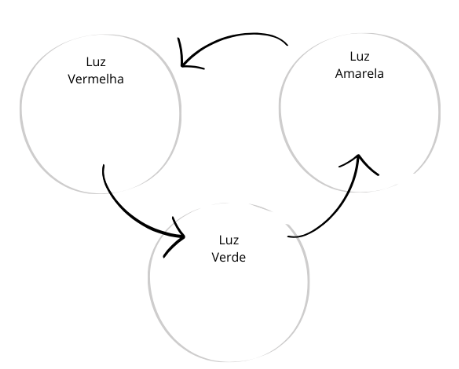
\includegraphics[width=0.5\linewidth]{circuitoMoore/semaforo.png}
    \caption{Máquina de Estados de um Semáforo}
    \label{fig:semaforo}
\end{figure}

O diagrama da Figura \ref{fig:semaforo} representa a máquina de estados que coordena a lógica de funcionamento de um semáforo. O sistema alterna entre três estados:

\begin{itemize}
    \item \textbf{Luz Vermelha:} Indica que o fluxo é proibido.
    \item \textbf{Luz Verde:} Permite o fluxo de veículos. 
    \item \textbf{Luz Amarela:} Um estado intermediário de curta duração que sinaliza o encerramento do fluxo. 
\end{itemize}
A Máquina inicia no \textbf{Estado de Luz Vermelha}, passa para o \textbf{Estado de Luz Verde}, segue para o \textbf{Estado de Luz Amarela}, e por fim retorna ao \textbf{Estado de Luz Vermelha} reiniciando o ciclo novamente.

\subsubsection{Implementação do circuíto lógico}

Como circuitos digitais usam binário, precisamos utilizar Flip-Flops para armazenar o estado atual. A cada Flip-Flop adicionado ao circuito dobramos a quantidade de \textbf{estados possíveis}. Assim, como necessitamos de 3 estados \textbf{(Luz Vermelha, Luz Amarela, Luz Verde)}, precisamos utilizar 2 Flip-Flops:
$2^1 < 3 < 2^2$

Após isso, contruimos a tabela com os respectivos estados:

\begin{table}[h]
    \centering
    \begin{tabular}{|l|c|c|}
    \hline
    \textbf{Estado Atual} & \textbf{Código Binário ($E_1 E_0)$} & Explicação\\
    \hline
    Vermelho & 00 & Ambos os Flip-Flops desligados \\
    Verde & 01 & Apenas o Flip-Flop 0 ($E_0$) ligado \\
    Amarelo & 10 & Apenas o Flip-Flop 1 ($E_1$) ligado \\
    \hline
    \end{tabular}
    \caption{Tabela representando os estados e seus respectivos códigos}
    \label{tab:semáforo}
\end{table}

\begin{tcolorbox}[mynote, title=Observação sobre o Estado 11 ser inutilizado] 
O estado 11 (ambos os Flip-Flops ligados) não é utilizado e é considerante irreleante \textbf{(Don't Care)}, pois só necessitamos de 3 estados para o funcionamento correto do circuito. Isso permite simplificar as equações booleanas.
\end{tcolorbox} 

\vspace{0.5em}

Após definir os códigos binários para cada estado, definiremos a lógica de transição. Esta tabela é fundamental para determinar as equações booleanas que controlarão a entrada dos \textbf{Flip-flops} ($E_1$ e $E_0$) e o acionamento das \textbf{lâmpadas} (Vermelha, Amarela e Verde)


\begin{table}[h]
    \centering
    \begin{tabular}{|c c|c c|c|c|c|}
    \hline
    \multicolumn{2}{|c|}{\textbf{Estado Atual}} & \multicolumn{2}{c|}{\textbf{Próximo Estado}} & \multicolumn{3}{c|}{\textbf{Saídas (Luzes)}} \\ \hline
    $E_1$ & $E_0$ & $E_1$ & $E_0$ & Vermelha & Verde & Amarela \\ \hline
    0 & 0 & 0 & 1 & 1 & 0 & 0 \\ \hline
    0 & 1 & 1 & 0 & 0 & 1 & 0 \\ \hline
    1 & 0 & 0 & 0 & 0 & 0 & 1 \\ \hline
    \end{tabular}
    \caption{Tabela da Transição de Estados e da Lógica da Saída}
    \label{tab:transicao_estados}
\end{table}

Após a construção da Tabela de Transição, o passo seguinte é extrair as equações booleanas das \textbf{saídas} e \textbf{entradas dos Flip-Flops}

\vspace{0.5em}
\textbf{Equações das Lâmpadas}

As lâmpadas dependem exclusivamente do estado atual ($E_1$ e $E_0$):

\begin{itemize}
    \item \textbf{Vermelha} = $\overline{E_1} \cdot \overline{E_0}$ (ativa apenas em 00)
    \item \textbf{Verde} = $ \overline{E_1} \cdot E_0$ (ativa apenas em 01)
    \item \textbf{Amarela} = $E_1 \cdot  \overline{E_0}$ (ativa apenas em 10) 
\end{itemize}

\vspace{0.5em}
\textbf{Equações dos Flip-Flops}

Para determinar qual será o estado seguinte para as entradas $D$ dos Flip-Flops,  olhamos para as colunas de "Próximo Estado":

\begin{itemize}
    \item \textbf{$D_1$} = $\overline{E_1} \cdot E_0$
    \item \textbf{$D_0$} = $\overline{E_1} \cdot \overline{E_0}$
\end{itemize}

\begin{figure}[H]
    \centering
    
    \begin{subfigure}{0.48\textwidth}
        \centering
        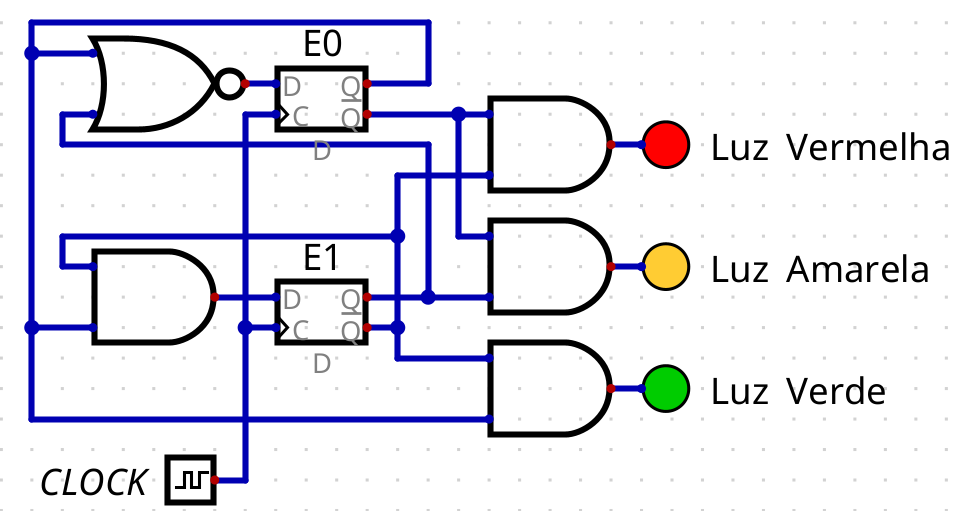
\includegraphics[width=\linewidth]{circuitoMoore/circuito.png}
        \caption*{Esquema lógico completo.}
    \end{subfigure}
    \hfill
    
    % Vermelho
    \begin{subfigure}{0.48\textwidth}
        \centering
        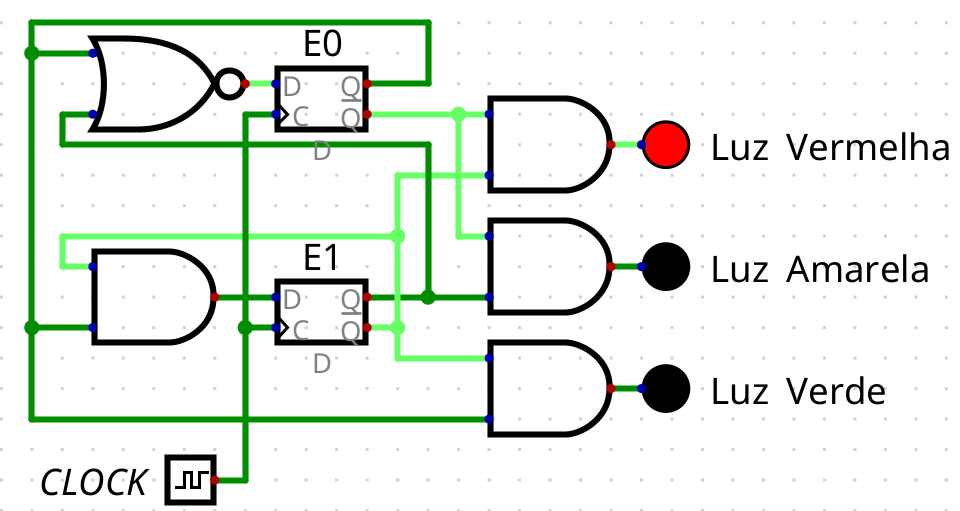
\includegraphics[width=\linewidth]{circuitoMoore/vermelho.png}
        \caption*{Estado 00: Luz Vermelha.}
    \end{subfigure}
    
    \vspace{1em}
    
    % Verde
    \begin{subfigure}{0.48\textwidth}
        \centering
        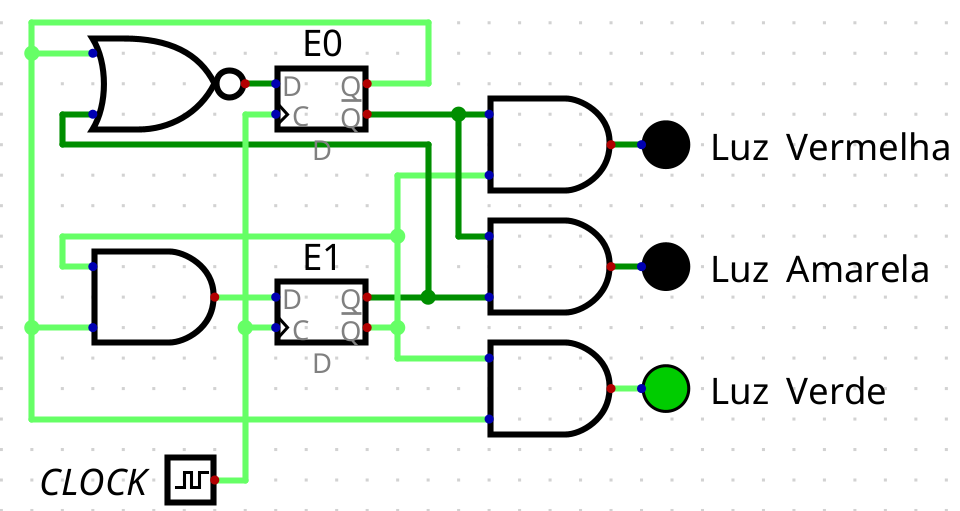
\includegraphics[width=\linewidth]{circuitoMoore/verde.png}
        \caption*{Estado 01: Luz Verde.}
    \end{subfigure}
    \hfill
    
    % Amarelo
    \begin{subfigure}{0.48\textwidth}
        \centering
        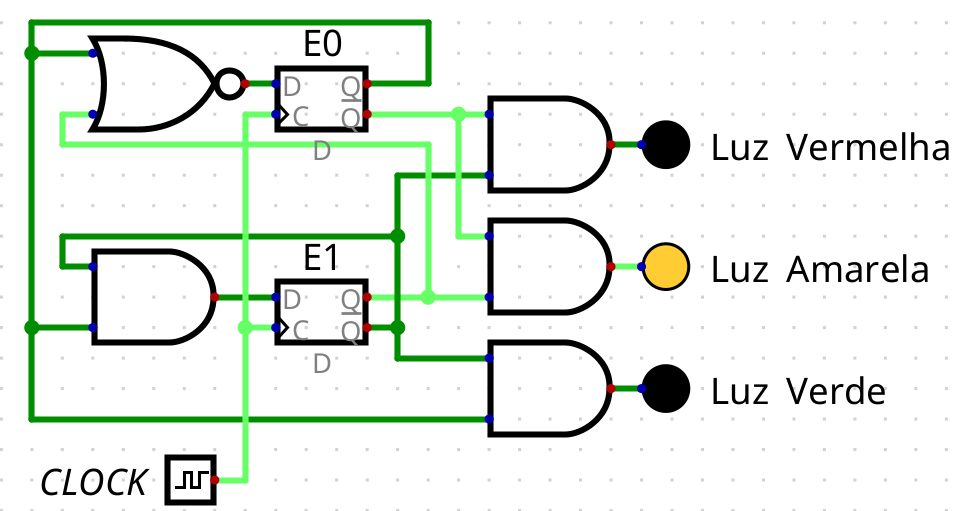
\includegraphics[width=\linewidth]{circuitoMoore/amarelo.png}
        \caption*{Estado 10: Luz Amarela.}
    \end{subfigure}
    
    \caption{Simulação do circuito lógico em funcionamento, monstrando a transição de estados e o acionamento das lâmpadas.}
    \label{fig:simulacao_completa}
\end{figure}

Observa-se que o circuito opera de forma cíclica e síncrona, onde cada combinação dos Flip-flops define o acionamento de uma única luz por vez. 

\subsection{Máquina de Mealy}

A Máquina de Mealy é outro tipo de máquina de estados que, diferente da Máquina de Moore, gera sua saída a partir da \textbf{combinação do estado atual com a entrada}. Isso significa que a saída pode ser alterada imediatamente sempre que houver una mudança na entrada, sem que ocorra uma mudança de estado.

Isso geralmente resulta em uma máquina de estado com um \textbf{número de estados reduzido} para realizar a mesma função, no entanto, a lógica para sua implementação tende a ser mais complexa.
\vspace{0.5em}
\textbf{Exemplo: Detector de Sequência}

\begin{figure}[h]
    \centering
    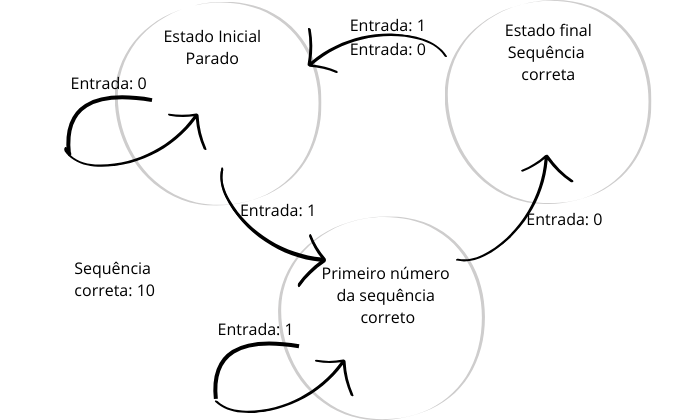
\includegraphics[width=0.5\linewidth]{circuitoMealy/mealy.png}
    \caption{Máquina de Estados de um Detector de Sequência}
    \label{fig:detector}
\end{figure}

O diagrama da Figura \ref{fig:detector} representa a máquina de estados que coordena a lógica de funcionamento de um detector de sequência. O sistema alterna entre três estados:

\begin{itemize}
    \item \textbf{Inicial/Parado:} Indica que não houve nenhuma entrada e/ou nenhuma entrada correta.
    \item \textbf{Primeiro número correto:} Indica que o primeiro número é correto. 
    \item \textbf{Final:} Indica que a sequência é a desejada. 
\end{itemize}

\subsubsection{Implementação do Detector de Sequência}

Para transpor o diagrama da Figura \ref{fig:detector} para um circuito digital, utilizaremos a codificação binária para os estados. Seguindo a mesma lógica utilizada no exemplo anterior do semáforo, como o sistema possui 3 estados, são necessários 2 Flip-Flops para a implementação do circuito. 
Uma possibilidade para os estados:

\begin{table}[H] 
\centering 
\begin{tabular}{|l|c|} 
\hline
\textbf{Estado} & \textbf{Código ($E_1$$E_0$)} \\ 
\hline
Inicial / Parado & 00 \\ 
Primeiro número correto (1) & 01 \\ Sequência correta (10) & 10 \\ 
\hline 
\end{tabular} 
\caption{Codificação de estados do detector de sequência.} 
\end{table}

\subsubsection{Tabela de Transição e Saída (Mealy)}

Diferente da abordagem de Moore utilizada no semáforo, a saída (S) neste circuito depende simultaneamente da entrada atual (X) e do estado atual. A tabela abaixo detalha como o sistema transita entre os estados e em que momento a sequência é validada:

\begin{table}[H] 
\centering 
\begin{tabular}{|c|cc|cc|c|} 
\hline 
\textbf{Entrada (X)} & \multicolumn{2}{c|}{\textbf{Estado Atual}} & \multicolumn{2}{c|}{\textbf{Próximo Estado}} & \textbf{Saída (S)} \\
\hline
X & $E_1$ & $E_0$ & $E_1$ & $E_0$ & S \\
0 & 0 & 0 & 0 & 0 & 0 \\
1 & 0 & 0 & 0 & 1 & 0 \\
0 & 0 & 1 & 1 & 0 & \textbf{1} \rlap{~$\longleftarrow$ \textbf{ Sequência "10" detectada!}} \\
1 & 0 & 1 & 0 & 1 & 0  \\ 
0 & 1 & 0 & 0 & 0 & 0  \\
1 & 1 & 0 & 0 & 0 & 0  \\
\hline
\end{tabular} 
\caption{Tabela de Transição e Lógica de Saída de Mealy.}
\end{table}

\subsubsection{Equações Booleanas}

A partir da Tabela de Transição, construimos as funções lógicas para as entradas dos Flip-Flops ($D_1$ e $D_0$) e para a saída (S). Nota-se que, por ser uma Máquina de Mealy, a variável de entrada X aparece diretamente na equação de saída:

\begin{itemize} 
    \item \textbf{$D_1$} = $\overline{E_1} \cdot E_0 \cdot \overline{X}$ (Acionado apenas quando o estado é "1" e chega o bit "0"). 
    \item \textbf{$D_0$} = $\overline{E_1} \cdot \overline{E_0} \cdot X$ + $\overline{E_1} \cdot E_0 \cdot X$ (Simplificado: o sistema permanece ou vai para o estado "1" sempre que a entrada for "1", desde que não esteja no estado final). 
    \item \textbf{Saída S} =$ \overline{E_1} \cdot E_0 \cdot X $
\end{itemize}

Observa-se que o detector de sequência apresenta uma resposta imediata assim que p bit "0" é detectado na entrada. Logo após isso a saída S assume nível lógico 1 sem aguardar a transição do próximo pulso de \textit{clock} para o estado final.

\subsubsection{Implementação do circuito lógico}
\begin{figure}[H]
    \centering
    
    \begin{subfigure}{0.48\textwidth}
        \centering
        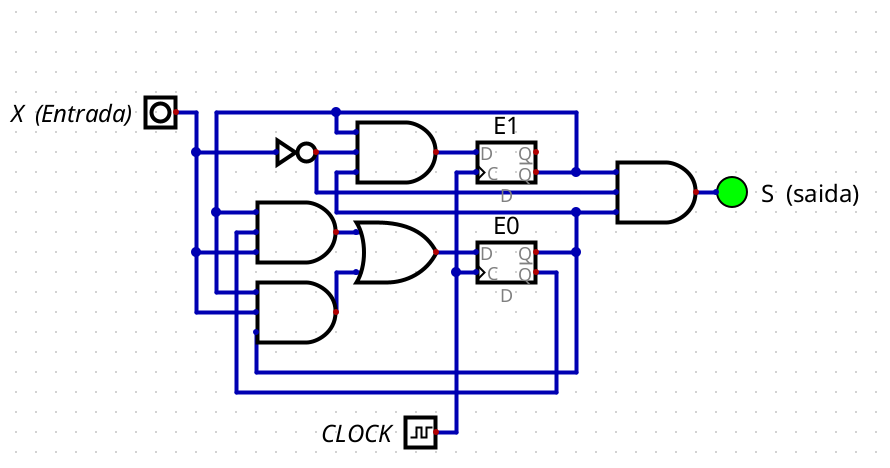
\includegraphics[width=\linewidth]{circuitoMealy/EstadoInativo.png}
        \caption*{Esquema lógico completo.}
    \end{subfigure}
    \hfill
    
    % Estado Inicial
    \begin{subfigure}{0.48\textwidth}
        \centering
        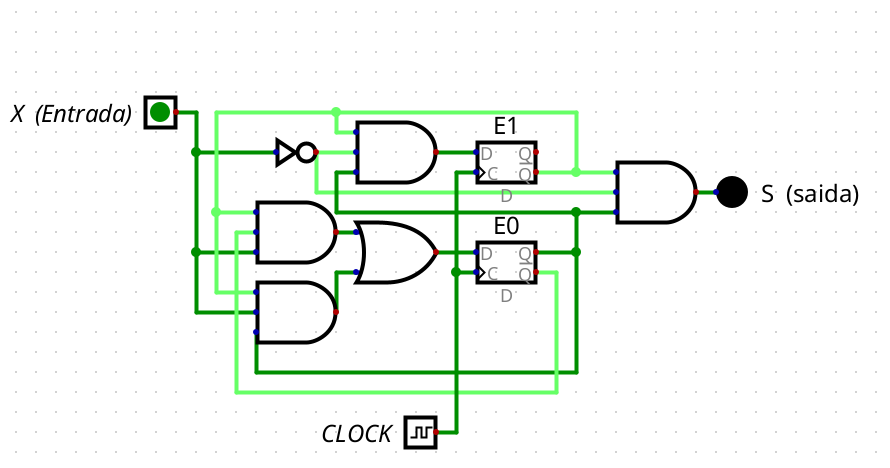
\includegraphics[width=\linewidth]{circuitoMealy/EstadoParado.png}
        \caption*{Estado 00: Inicial/Parado.}
    \end{subfigure}
    
    \vspace{1em}
    
    % Estado 1 Correto
    \begin{subfigure}{0.48\textwidth}
        \centering
        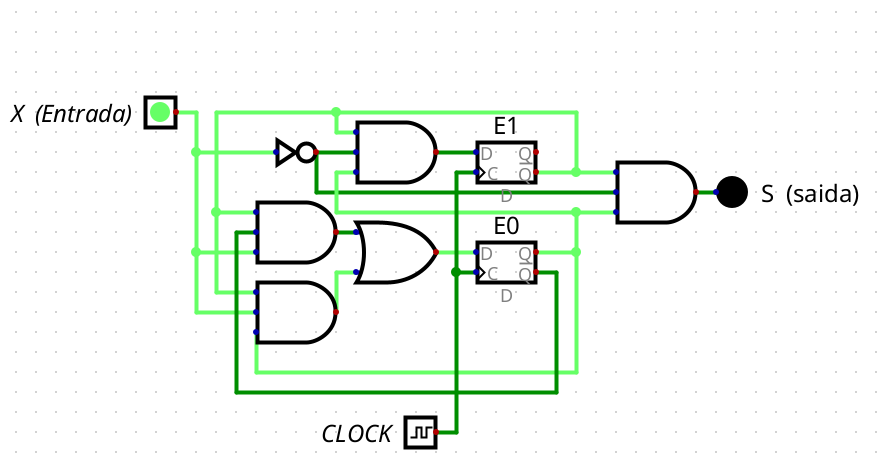
\includegraphics[width=\linewidth]{circuitoMealy/Estado1Correto.png}
        \caption*{Estado 01: 1º número correto.}
    \end{subfigure}
    \hfill
    
    % Estado Final
    \begin{subfigure}{0.48\textwidth}
        \centering
        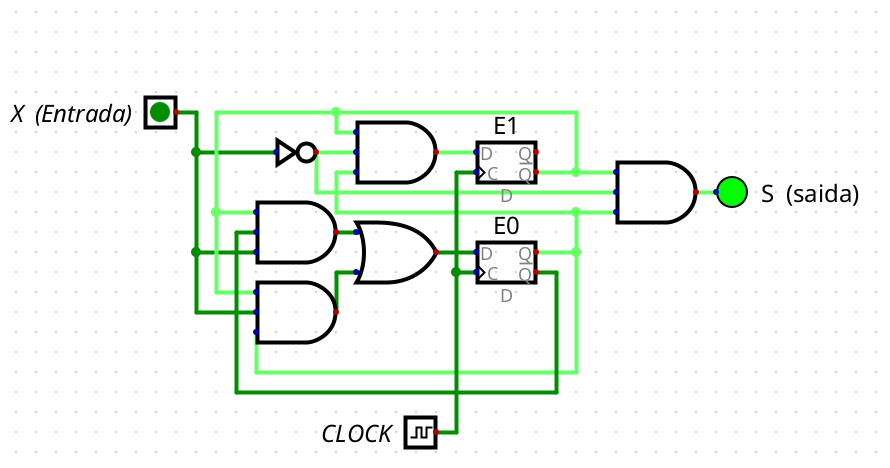
\includegraphics[width=\linewidth]{circuitoMealy/EstadoFinal.png}
        \caption*{Estado 10: Estado Final/ Sequência Correta.}
    \end{subfigure}
    
    \caption{Simulação do detector de sequência em funcionamento, destacando a ativação da saída $S$ no momento da detecção.}
    \label{fig:simulacao_completa_mealy}
\end{figure}

O circuito acima comprova que a Máquina de Mealy responde instantaneamente às variações da entrada. Diferente do semáforo, a saída deste detector ativa imediatamente assim que a sequência "10" é completada, sem depender de um próximo \textit{clock}.

\end{document}


